\section{Resultados} \label{resultados}

\subsection{Número de ejecuciones y validación}

Para la ejecución de nuestros algoritmos separaremos los conjuntos de datos en dos partes, una de entrenamiento y otra de test, utilizando un $80\%$ del conjunto para el entrenamiento y el $20\%$ restante para el test.

De cara a validar los resultados, se ha utilizado la validación 5x2cv explicada con anterioridad sobre el conjunto de entrenamiento obtenido.

También tenemos que tener en cuenta que los algoritmos implementados son algoritmos estocásticos, es decir, la aleatoriedad juega una parte importante en las zonas del espacio de soluciones que se explorarán, por este motivo se han realizado cinco ejecuciones distintas, con cinco semillas aleatorias distintas.

\subsection{Parámetros utilizados}

Como vimos en el estado del arte, la Programación Genética es un algoritmo que necesita una población con un gran número de individuos, por este motivo se ha escogido una población de mil individuos. De cara a estudiar el sobreajuste de las expresiones y mantener el resultado simple se ha experimentado con distintas longitudes máximas de nodos, variando entre veinte, cuarenta y sesenta. Se ha tomado el valor inicial veinte ya que contamos con nueve nodos, y una expresión en la que intervengan todos los nodos con una única operación ya supondría una longitud de árbol de dicho tamaño.

Con respecto a los demás parámetros se han utilizado los más comunes en otras implementaciones de Programación Genética y que de forma empírica han funcionado mejor en nuestro conjunto de datos.

Se han utilizado los siguientes parámetros:

\begin{itemize}
	\item Tamaño de población: $1.000$.
	\item Probabilidad de que un nodo sea una variable: $30\%$.
	\item Tamaño máximo del árbol: $20$, $40$ y $60$.
	\item Número de evaluaciones: $1.000.000$.
	\item Probabilidad de cruce en PG: $75\%$.
	\item Probabilidad de cruce en GA (solo para GA-P): $75\%$.
	\item Probabilidad de mutación en PG: $5\%$.
	\item Probabilidad de mutación en GA (solo para GA-P): $5\%$.
	\item Probabilidad de cruce intra-nicho (solo para GA-P): $40\%$.
	\item Tamaño del torneo: $100$.
\end{itemize}

\newpage

\subsection{Resultados de Programación Genética en el conjunto de datos original}

Tras las distintas ejecuciones con las semillas aleatorias, en cada uno de los conjuntos de datos y con distintas profundidades máximas para las expresiones, obtenemos los siguientes resultados.


\subsubsection{Resultados en la lateralidad izquierda}

% Please add the following required packages to your document preamble:
% \usepackage{graphicx}
\begin{table}[H]
\centering
\resizebox{\textwidth}{!}{%
\begin{tabular}{|c|c|c|c|c|}
\hline
\multicolumn{5}{|c|}{\textbf{Produndidad máxima: 20}}                                                                        \\ \hline
\textbf{Semilla} & \textbf{ECM con 5x2-cv} & \textbf{RECM con 5x2cv} & \textbf{MAE con 5x2cv} & \textbf{Tiempo de ejecución (s)} \\ \hline
8324             & 79,9537                 & 8,9389                  & 7,46834                & 211,958                      \\ \hline
12345            & 80,3763                 & 8,9594                  & 7,5213                 & 211,641                      \\ \hline
34634            & 78,5994                 & 8,86191                 & 7,31334                & 212,611                      \\ \hline
34679            & 79,6023                 & 8,91243                 & 7,36373                & 210,634                      \\ \hline
92034            & 72,9244                 & 8,53155                 & 7,07619                & 211,236                      \\ \hline
\textbf{Media}   & \textbf{78,29122}       & \textbf{8,840838}       & \textbf{7,34858}       & \textbf{211,616}             \\ \hline
\end{tabular}%
}
\caption{Resultados de Programación Genética en la lateralidad izquierda con cinco semillas distintas y una profundidad máxima de 20 nodos.}\label{table:resultados_PG_l0_20}
\end{table}



% Please add the following required packages to your document preamble:
% \usepackage{graphicx}
\begin{table}[H]
\centering
\resizebox{\textwidth}{!}{%
\begin{tabular}{|c|c|}
\hline
\multicolumn{2}{|c|}{\textbf{Produndidad máxima: 20}}                                                                                         \\ \hline
\textbf{Semilla} & \textbf{Expresión simplificada}                                                                                            \\ \hline
8324             & $9,974419 x_{4} + \left(- x_{6} + x_{8} + 2,969837\right) \left(- 0,212752422771402 x_{0} x_{1} + x_{1} + 3,804588\right)$ \\ \hline
12345            & $\frac{x_{2} \left(x_{4} + x_{7} + x_{8}\right) + 3,222534 x_{4}^{2} x_{6} \left(x_{1} + 4,282022\right)}{x_{4} x_{6}}$    \\ \hline
34634            & $x_{7} - \left(x_{0} - 6,300796\right) \left(x_{0} x_{1} + 0,60016361304954 x_{8} + 4,741612\right)$                       \\ \hline
34679            & $x_{4} \left(x_{1} - x_{4} - 2 x_{6} + 2 x_{8} + 18,187769\right)$                                                         \\ \hline
92034            & $x_{4} \left(x_{4} x_{6} \left(x_{1} - 3,032651\right) + 2,64098115386946 x_{8} + 17,1523961459229\right)$                 \\ \hline
\end{tabular}%
}
\caption{Expresiones obtenidas con Programación Genética en la lateralidad izquierda con cinco semillas distintas y una profundidad máxima de 20 nodos.}\label{table:exp_PG_l0_20}
\end{table}



% Please add the following required packages to your document preamble:
% \usepackage{graphicx}
\begin{table}[H]
\centering
\resizebox{\textwidth}{!}{%
\begin{tabular}{|c|c|c|c|c|}
\hline
\multicolumn{5}{|c|}{\textbf{Produndidad máxima: 40}}                                                                        \\ \hline
\textbf{Semilla} & \textbf{ECM con 5x2-cv} & \textbf{RECM con 5x2cv} & \textbf{MAE con 5x2cv} & \textbf{Tiempo de ejecución (s)} \\ \hline
8324             & 77,4991                 & 8,79915                 & 7,35549                & 371,394                      \\ \hline
12345            & 113,413                 & 10,0316                 & 7,44315                & 376,57                       \\ \hline
34634            & 77,0115                 & 8,76665                 & 7,22587                & 367,263                      \\ \hline
34679            & 77,1488                 & 8,78025                 & 7,25083                & 376,047                      \\ \hline
92034            & 72,6009                 & 8,5159                  & 7,13994                & 377,999                      \\ \hline
\textbf{Media}   & \textbf{83,53466}       & \textbf{8,97871}        & \textbf{7,283056}      & \textbf{373,8546}            \\ \hline
\end{tabular}%
}
\caption{Resultados de Programación Genética en la lateralidad izquierda con cinco semillas distintas y una profundidad máxima de 40 nodos.}\label{table:resultados_PG_l0_40}

\end{table}


% Please add the following required packages to your document preamble:
% \usepackage{graphicx}
\begin{table}[H]
\centering
\resizebox{\textwidth}{!}{%
\begin{tabular}{|c|c|}
\hline
\multicolumn{2}{|c|}{\textbf{Produndidad máxima: 40}}                                                                                                                                                                                                                              \\ \hline
\textbf{Semilla} & \textbf{Expresión simplificada}                                                                                                                                                                                                                                 \\ \hline
8324             & $2,64567680120389 x_{1} + x_{4} \left(\frac{x_{1}}{x_{7}} + x_{7} + 9,746081\right) + 4,05969285034077 x_{8} + \frac{6,861339}{x_{1} \left(x_{7} - 2,180585\right) + 2 x_{6} - x_{7} + 2,884742}$                                                               \\ \hline
12345            & $\frac{x_{1} x_{8} + x_{7} \left(x_{4} - x_{7}\right) + x_{8} \left(x_{4} - x_{7}\right) \left(x_{4} - x_{6} + 2 x_{7} - \left(0,679759280540821 x_{0} - x_{8}\right) \left(x_{1} + 3,45996\right) + 27,341369407935\right)}{x_{8} \left(x_{4} - x_{7}\right)}$ \\ \hline
34634            & $\frac{54,02429862327 x_{2} x_{6}^{4} + \left(1,922931 x_{2} x_{6}^{5} + 1,20955523302424\right) \left(- x_{0} + x_{1}^{2} + x_{4} \left(x_{1} + x_{8} + 6,523721\right)\right)}{1,922931 x_{2} x_{6}^{5} + 1,20955523302424}$                                  \\ \hline
34679            & $x_{1} \left(\frac{x_{5}}{x_{0} + x_{4} - x_{8} - 4,554789 + \frac{5,549382}{x_{6} x_{8}}} + 3,773635\right) + x_{4} \left(2 x_{8} + 10,486591\right) + \frac{5,361796}{x_{0} x_{6}}$                                                                           \\ \hline
92034            & $\frac{x_{7} x_{8} \left(x_{7} - 5,534974\right) + \left(- x_{1} + x_{8} \left(13,8664710431387 x_{4} + 11,584123\right)\right) \left(0,114592928103709 x_{1} + 0,114592928103709 x_{8} + 0,79479225562657\right)}{x_{8}}$                                      \\ \hline
\end{tabular}%
}
\caption{Expresiones obtenidas con Programación Genética en la lateralidad izquierda con cinco semillas distintas y una profundidad máxima de 40 nodos.}\label{table:exp_PG_l0_40}
\end{table}





% Please add the following required packages to your document preamble:
% \usepackage{graphicx}
\begin{table}[H]
\centering
\resizebox{\textwidth}{!}{%
\begin{tabular}{|c|c|c|c|c|}
\hline
\multicolumn{5}{|c|}{\textbf{Produndidad máxima: 60}}                                                                        \\ \hline
\textbf{Semilla} & \textbf{ECM con 5x2-cv} & \textbf{RECM con 5x2cv} & \textbf{MAE con 5x2cv} & \textbf{Tiempo de ejecución (s)} \\ \hline
8324             & 76,673                  & 8,75413                 & 7,23217                & 522,304                      \\ \hline
12345            & 83,7292                 & 9,1046                  & 7,38679                & 516,579                      \\ \hline
34634            & 77,2803                 & 8,78271                 & 7,24127                & 519,752                      \\ \hline
34679            & 78,6668                 & 8,85517                 & 7,29779                & 523,821                      \\ \hline
92034            & 74,9574                 & 8,64884                 & 7,16493                & 517,639                      \\ \hline
\textbf{Media}   & \textbf{78,26134}       & \textbf{8,82909}        & \textbf{7,26459}       & \textbf{520,019}             \\ \hline
\end{tabular}%
}
\caption{Resultados de Programación Genética en la lateralidad izquierda con cinco semillas distintas y una profundidad máxima de 60 nodos.}\label{table:resultados_PG_l0_60}

\end{table}

% Please add the following required packages to your document preamble:
% \usepackage{graphicx}
\begin{table}[H]
\centering
\resizebox{\textwidth}{!}{%
\begin{tabular}{|c|c|}
\hline
\multicolumn{2}{|c|}{\textbf{Produndidad máxima: 60}}                                                                                                                                                                                                                                                                                                                                                                                                                  \\ \hline
\textbf{Semilla} & \textbf{Expresión simplificada}                                                                                                                                                                                                                                                                                                                                                                                                                     \\ \hline
8324             & $63,37721638562 + \frac{x_{0} \left(11,0360508048173 - \frac{2,91178457453004 x_{8}}{x_{7}}\right) + 2,11060529318769 x_{6} - 2,11060529318769 x_{8} - \frac{8,463155}{x_{7}} + \frac{54,8941311814834}{x_{7} \left(3,788494 x_{1} - x_{4}\right)}}{0,280491324650179 x_{4}^{2} x_{6} - 4,20445} - \frac{30,1726087626953}{x_{4}}$                                                                                                                  \\ \hline
12345            & $1,37381094513708 x_{0} + x_{1} - \left(\frac{19,712441757483 x_{0}}{x_{1} \left(- 9,202272 x_{5} + 27,493011502176 x_{8} + 20,641966009536\right)} - 4,75549\right) \left(9,312897 - \frac{0,554589645256733 x_{6}^{2}}{x_{1}} + \frac{x_{8} - 2,443419}{x_{0}^{3} x_{7}}\right) - 0,339968$                                                                                                                                                       \\ \hline
34634            & $\frac{x_{0} x_{7} \left(- 1,70984801423089 x_{1} + 1,93398737553041 x_{8} + 9,50115349702912\right) + 1,26779026692056 x_{4} \left(x_{0} x_{7} \left(x_{1} + 8,552745\right) + x_{0} \left(2,5671379346047 x_{1} + 0,573141861980187 x_{8} - 4,07495666904651\right) + x_{7}^{2}\right)}{x_{0} x_{7}}$                                                                                                                                             \\ \hline
34679            & $\frac{3,262489 x_{0}}{0,814551165671653 x_{0} - \frac{- x_{0} + \left(4,330122 x_{6} - 3,020402989026\right) \left(2,785333 x_{8} - 3,889542058521\right) + \frac{x_{8}}{x_{0}^{2}}}{x_{6}}} - 1,28453905858423 x_{1} + 70,0029154694077 - \frac{36,228540737219}{x_{8}} - \frac{13,671283980094}{x_{1}}$                                                                                                                                          \\ \hline
92034            & $\frac{\left(x_{6} - 9,999223\right) \left(\left(x_{0} - 9,809002\right) \left(x_{0} - 5,03568\right) + 6,736629\right) \left(\left(6,022963 x_{0} - 26,510041261783\right) \left(2,020491 x_{0} + x_{1} + x_{6} + 10,71872986848\right) + \left(x_{1} - 3,013815\right) \left(x_{8} - 9,809002\right)\right)}{\left(x_{0} - 9,809002\right) \left(6,022963 x_{0} - 26,510041261783\right) \left(2,64667191228567 x_{6} + 11,5238525972231\right)}$ \\ \hline
\end{tabular}%
}
\caption{Resultados de Programación Genética en la lateralidad izquierda con cinco semillas distintas y una profundidad máxima de 60 nodos.}\label{table:exp_PG_l0_60}
\end{table}



\subsubsection{Resultados en la lateralidad derecha}


% Please add the following required packages to your document preamble:
% \usepackage{graphicx}
\begin{table}[H]
\centering
\resizebox{\textwidth}{!}{%
\begin{tabular}{|c|c|c|c|c|}
\hline
\multicolumn{5}{|c|}{\textbf{Produndidad máxima: 20}}                                                                            \\ \hline
\textbf{Semilla} & \textbf{ECM con 5x2-cv} & \textbf{RECM con 5x2cv} & \textbf{MAE con 5x2cv} & \textbf{Tiempo de ejecución (s)} \\ \hline
8324             & 72,3476                 & 8,50209                 & 6,99355                & 215,559                          \\ \hline
12345            & 70,884                  & 8,41339                 & 6,86307                & 213,978                          \\ \hline
34634            & 74,9666                 & 8,64992                 & 7,10458                & 211,862                          \\ \hline
34679            & 74,7413                 & 8,63821                 & 7,118                  & 210,305                          \\ \hline
92034            & 67,5138                 & 8,21472                 & 6,73837                & 213,598                          \\ \hline
\textbf{Media}   & \textbf{72,09066}       & \textbf{8,483666}       & \textbf{6,963514}      & \textbf{213,0604}                \\ \hline
\end{tabular}%
}
\caption{Resultados de Programación Genética en la lateralidad derecha con cinco semillas distintas y una profundidad máxima de 20 nodos.}\label{table:resultados_PG_l1_20}
\end{table}

% Please add the following required packages to your document preamble:
% \usepackage{graphicx}
\begin{table}[H]
\centering
\resizebox{\textwidth}{!}{%
\begin{tabular}{|c|c|}
\hline
\multicolumn{2}{|c|}{\textbf{Produndidad máxima: 20}}                                                                                                               \\ \hline
\textbf{Semilla} & \textbf{Expresión simplificada}                                                                                                                  \\ \hline
8324             & $- x_{0} + x_{1} + 6.256587 x_{4} - x_{7} + 6.256587 x_{8} + 15.413785997178 - \frac{x_{7}}{x_{1}}$                                              \\ \hline
12345            & $\frac{2.964502 x_{1}}{x_{7}} + 9.709103 x_{4} x_{5} + 3 x_{8} - 5.833099$                                                                       \\ \hline
34634            & $- x_{1} \left(- 7.559452 x_{4} + x_{8} + 6.724939\right) + 7.559452 x_{8} + 12.549552$                                                          \\ \hline
34679            & $\frac{- x_{7} x_{8} \left(x_{8} + 0.43834\right) + \left(x_{4} + x_{8}\right) \left(- 0.489073 x_{0} + 9.97633 x_{7} + 2.139935\right)}{x_{7}}$ \\ \hline
92034            & $\frac{x_{4} x_{8} \left(8.345482 x_{8} + 24.346950622642\right) - 4.674466 x_{8} \left(- x_{1} + x_{8}\right) - 11.865982358088}{x_{4} x_{8}}$  \\ \hline
\end{tabular}%
}
\caption{Expresiones obtenidas con Programación Genética en la lateralidad derecha con cinco semillas distintas y una profundidad máxima de 20 nodos.}\label{table:exp_PG_l1_20}

\end{table}




% Please add the following required packages to your document preamble:
% \usepackage{graphicx}
\begin{table}[H]
\centering
\resizebox{\textwidth}{!}{%
\begin{tabular}{|c|c|c|c|c|}
\hline
\multicolumn{5}{|c|}{\textbf{Produndidad máxima: 40}}                                                                            \\ \hline
\textbf{Semilla} & \textbf{ECM con 5x2-cv} & \textbf{RECM con 5x2cv} & \textbf{MAE con 5x2cv} & \textbf{Tiempo de ejecución (s)} \\ \hline
8324             & 72,0551                 & 8,48533                 & 6,95435                & 388,36                           \\ \hline
12345            & 70,7415                 & 8,40321                 & 6,87752                & 391,053                          \\ \hline
34634            & 74,7811                 & 8,64441                 & 7,08979                & 390,666                          \\ \hline
34679            & 72,4849                 & 8,50504                 & 6,95179                & 389,966                          \\ \hline
92034            & 68,3543                 & 8,26171                 & 6,7361                 & 396,093                          \\ \hline
\textbf{Media}   & \textbf{71,68338}       & \textbf{8,45994}        & \textbf{6,92191}       & \textbf{391,2276}                \\ \hline
\end{tabular}%
}
\caption{Resultados de Programación Genética en la lateralidad derecha con cinco semillas distintas y una profundidad máxima de 40 nodos.}\label{table:resultados_PG_l1_40}

\end{table}


% Please add the following required packages to your document preamble:
% \usepackage{graphicx}
\begin{table}[H]
\centering
\resizebox{\textwidth}{!}{%
\begin{tabular}{|c|c|}
\hline
\multicolumn{2}{|c|}{\textbf{Produndidad máxima: 40}}                                                                                                                                                                                                                                                                                                                                                                              \\ \hline
\textbf{Semilla} & \textbf{Expresión simplificada}                                                                                                                                                                                                                                                                                                                                                                                 \\ \hline
8324             & $\frac{x_{4} \left(x_{4} + 1.916243 \left(x_{1} - 1.819181\right) \left(x_{8} + 8.079178\right) \left(x_{3} \left(3.031727 x_{1} - 9.94007728148587\right) + 0.662162\right) \left(8.079178 x_{3} + x_{4} - x_{8} - 9.332657\right)\right)}{\left(x_{1} - 1.819181\right) \left(x_{3} \left(3.031727 x_{1} - 9.94007728148587\right) + 0.662162\right) \left(8.079178 x_{3} + x_{4} - x_{8} - 9.332657\right)}$ \\ \hline
12345            & $\frac{x_{2} \left(x_{0} - 2.381496\right) \left(- x_{2} + 3.864150735106 x_{4} \left(x_{2} + x_{5}\right) - 2.576954 x_{4} + x_{7} + 4.864150735106 x_{8} + 4.860383\right) - x_{4} x_{7} \left(x_{1} - x_{5}\right)}{x_{2} \left(x_{0} - 2.381496\right)}$                                                                                                                                                    \\ \hline
34634            & $x_{5} \left(- 0.067246 x_{0} + 0.932754 x_{1} - 0.537787242752 x_{4} x_{6} + 6.223157 x_{4} + x_{5} x_{8} - 0.067246 x_{7} + x_{8} + 0.991449587285935\right)$                                                                                                                                                                                                                                                 \\ \hline
34679            & $\frac{- x_{1} \left(x_{8} + 4.573654\right) + \left(x_{1} x_{4} - 0.578333497692\right) \left(x_{1} x_{2} + x_{1} + 5.801173 x_{8} + 25.6274319346107\right)}{x_{1} x_{4} - 0.578333497692}$                                                                                                                                                                                                                   \\ \hline
92034            & $\frac{x_{8} \left(x_{4} x_{8}^{2} + \left(0.103744028623392 x_{1} x_{6} \left(x_{1} + x_{8} - 7.15049\right) - 0.866056935799694\right) \left(x_{1} - x_{7} + 7.489655\right) \left(x_{1} + x_{6} - x_{8} + 17.734692\right)\right)}{\left(0.103744028623392 x_{1} x_{6} \left(x_{1} + x_{8} - 7.15049\right) - 0.866056935799694\right) \left(x_{1} - x_{7} + 7.489655\right)}$                               \\ \hline
\end{tabular}%
}
\caption{Expresiones obtenidas con Programación Genética en la lateralidad derecha con cinco semillas distintas y una profundidad máxima de 40 nodos.}\label{table:exp_PG_l1_40}
\end{table}





\begin{table}[H]
\centering
\resizebox{\textwidth}{!}{%
\begin{tabular}{|c|c|c|c|c|}
\hline
\multicolumn{5}{|c|}{\textbf{Produndidad máxima: 60}}                                                                            \\ \hline
\textbf{Semilla} & \textbf{ECM con 5x2-cv} & \textbf{RECM con 5x2cv} & \textbf{MAE con 5x2cv} & \textbf{Tiempo de ejecución (s)} \\ \hline
8324             & 77,6228                 & 8,79922                 & 7,10807                & 534,707                          \\ \hline
12345            & 68,9063                 & 8,29117                 & 6,73511                & 545,115                          \\ \hline
34634            & 74,2657                 & 8,61588                 & 7,11258                & 507,235                          \\ \hline
34679            & 87,2423                 & 9,10656                 & 7,10872                & 537,105                          \\ \hline
92034            & 71,1911                 & 8,42445                 & 6,81426                & 541,437                          \\ \hline
\textbf{Media}   & \textbf{75,84564}       & \textbf{8,647456}       & \textbf{6,975748}      & \textbf{533,1198}                \\ \hline
\end{tabular}%
}
\caption{Resultados de Programación Genética en la lateralidad derecha con cinco semillas distintas y una profundidad máxima de 60 nodos.}\label{table:resultados_PG_l1_60}

\end{table}

% Please add the following required packages to your document preamble:
% \usepackage{graphicx}
\begin{table}[H]
\centering
\resizebox{\textwidth}{!}{%
\begin{tabular}{|c|c|}
\hline
\multicolumn{2}{|c|}{\textbf{Produndidad máxima: 60}}                                                                                                                                                                                                                                                                                                                                                                                                                                        \\ \hline
\textbf{Semilla} & \textbf{Expresión simplificada}                                                                                                                                                                                                                                                                                                                                                                                                                                           \\ \hline
8324             & $- x_{1} - x_{7} + 3 x_{8} + \frac{1.190954 + \frac{6.872244}{x_{6}}}{-12.148502 + \frac{x_{7} + 1.908513}{x_{5} - 0.727969000000001} + \frac{8.931837}{x_{4}}} + 34.386611 - \frac{9.262717}{x_{8}} + \frac{6.356476 x_{1}}{x_{0}}$                                                                                                                                                                                                                                      \\ \hline
12345            & $\frac{x_{4}^{2} x_{6} \left(7.055295 x_{7} - 4.125957\right) \left(- x_{0} + x_{8} + 17.78709\right) + x_{7} \left(0.251984821442296 x_{1} - 3.54182051880298\right) \left(0.606888580149495 x_{1} \left(0.250525602714495 x_{1} - 3.24847625695108\right) \left(x_{6} \left(x_{8} + 2.010911\right) + 2.833802\right) + x_{4} x_{6} \left(x_{7} - x_{8} + 4.058117\right)\right)}{x_{4} x_{6} \left(7.055295 x_{7} - 4.125957\right)}$                                  \\ \hline
34634            & $\frac{137.833269053922 x_{8} \left(- 7.578356 x_{1} + \left(x_{2} + 7.529862\right) \left(x_{7} + 1.638587\right) + 6.195498\right) + \left(2 x_{6} + 1.48736466964042\right) \left(x_{7} + 1.638587\right) \left(7.732896 x_{7} + 55.356338126592\right) \left(7.578356 x_{1} + x_{4} \left(x_{4} x_{6} + 7.32304\right) + 0.311624993336\right)}{\left(2 x_{6} + 1.48736466964042\right) \left(x_{7} + 1.638587\right) \left(7.732896 x_{7} + 55.356338126592\right)}$ \\ \hline
34679            & $\frac{x_{6} \left(x_{4} - x_{7} + 3.25889177193228 x_{8} - \left(2.41698871433944 x_{1} - 1.059771\right) \left(x_{8} - 4.617387\right)\right) + \left(7.56949 x_{4} + 2.822881\right) \left(x_{6} \left(0.171871788831501 x_{2} + 0.171871788831501 x_{8} + 0.406220519749351\right) + 0.429802532279555\right)}{x_{6}}$                                                                                                                                                \\ \hline
92034            & $\frac{\left(7.98415134817207 x_{8} - 4.86642\right) \left(x_{7} \left(2.676506 x_{0} - 157.560604751895\right) - 0.282392155665583 x_{8} \left(4.937414 x_{7} + 9.97651\right)\right)}{x_{7} \left(x_{1} + x_{8} \left(1.52743497395565 x_{1} - 26.5940100612299\right)\right)}$                                                                                                                                                                                         \\ \hline
\end{tabular}%
}
\caption{Expresiones obtenidas con Programación Genética en la lateralidad derecha con cinco semillas distintas y una profundidad máxima de 60 nodos.}\label{table:exp_PG_l1_60}
\end{table}



\subsubsection{Resultados en el conjunto completo}

% Please add the following required packages to your document preamble:
% \usepackage{graphicx}
\begin{table}[H]
\centering
\resizebox{\textwidth}{!}{%
\begin{tabular}{|c|c|c|c|c|}
\hline
\multicolumn{5}{|c|}{\textbf{Produndidad máxima: 20}}                                                                            \\ \hline
\textbf{Semilla} & \textbf{ECM con 5x2-cv} & \textbf{RECM con 5x2cv} & \textbf{MAE con 5x2cv} & \textbf{Tiempo de ejecución (s)} \\ \hline
8324             & 75,1256                 & 8,66525                 & 7,12232                & 344,445                          \\ \hline
12345            & 73,594                  & 8,57715                 & 7,08578                & 342,743                          \\ \hline
34634            & 73,0808                 & 8,54466                 & 7,01207                & 359,184                          \\ \hline
34679            & 75,1162                 & 8,66306                 & 7,18915                & 353,337                          \\ \hline
92034            & 70,5851                 & 8,39821                 & 6,92052                & 347,82                           \\ \hline
\textbf{Media}   & \textbf{73,50034}       & \textbf{8,569666}       & \textbf{7,065968}      & \textbf{349,5058}                \\ \hline
\end{tabular}%
}
\caption{Resultados de Programación Genética en el conjunto de datos completo con cinco semillas distintas y una profundidad máxima de 20 nodos.}\label{table:resultados_PG_c_20}
\end{table}

% Please add the following required packages to your document preamble:
% \usepackage{graphicx}
\begin{table}[H]
\centering
\resizebox{\textwidth}{!}{%
\begin{tabular}{|c|c|}
\hline
\multicolumn{2}{|c|}{\textbf{Produndidad máxima: 20}}                                                                                                          \\ \hline
\textbf{Semilla} & \textbf{Expresión simplificada}                                                                                                             \\ \hline
8324             & $\frac{x_{6} \left(11,085082 - x_{0}\right) + \left(x_{1} + 8,10638\right) \left(x_{4} x_{6} + 0,52645848743212 x_{8}\right)}{x_{6}}$       \\ \hline
12345            & $\frac{0,13644040890099 x_{4} \left(21,30535985094 x_{1} - x_{8}\right) \left(5,128064 x_{3} + 1,15335730778724 x_{8}\right)}{x_{1} x_{3}}$ \\ \hline
34634            & $8,739828 x_{4} + 5,21414207782618 x_{8} + 7,225131 + \frac{2,341281 x_{1}}{x_{0}}$                                                         \\ \hline
34679            & $\frac{3,354085 x_{0} x_{1} + \left(5,58451 x_{0} x_{1} - 1,123423\right) \left(- x_{0} + x_{8} + 6,704773\right)}{x_{0} x_{1}}$            \\ \hline
92034            & $10,856454 x_{4} + 5,428227 x_{8} + 8,374907 - \frac{3,803607512943}{x_{1}^{3}}$                                                            \\ \hline
\end{tabular}%
}
\caption{Expresiones obtenidas con Programación Genética en el conjunto de datos completo con cinco semillas distintas y una profundidad máxima de 20 nodos.}\label{table:exp_PG_c_20}

\end{table}


% Please add the following required packages to your document preamble:
% \usepackage{graphicx}
\begin{table}[H]
\centering
\resizebox{\textwidth}{!}{%
\begin{tabular}{|c|c|c|c|c|}
\hline
\multicolumn{5}{|c|}{\textbf{Produndidad máxima: 40}}                                                                            \\ \hline
\textbf{Semilla} & \textbf{ECM con 5x2-cv} & \textbf{RECM con 5x2cv} & \textbf{MAE con 5x2cv} & \textbf{Tiempo de ejecución (s)} \\ \hline
8324             & 75,368                  & 8,68014                 & 7,17403                & 665,789                          \\ \hline
12345            & 71,6442                 & 8,46147                 & 6,97584                & 652,943                          \\ \hline
34634            & 70,6075                 & 8,3956                  & 6,93068                & 660,407                          \\ \hline
34679            & 72,1347                 & 8,49127                 & 7,02663                & 683,528                          \\ \hline
92034            & 73,1519                 & 8,54904                 & 6,99538                & 651,94                           \\ \hline
\textbf{Media}   & \textbf{72,58126}       & \textbf{8,515504}       & \textbf{7,020512}      & \textbf{662,9214}                \\ \hline
\end{tabular}%
}
\caption{Resultados de Programación Genética en el conjunto de datos completo con cinco semillas distintas y una profundidad máxima de 40 nodos.}\label{table:resultados_PG_c_40}

\end{table}

% Please add the following required packages to your document preamble:
% \usepackage{graphicx}
\begin{table}[H]
\centering
\resizebox{\textwidth}{!}{%
\begin{tabular}{|c|c|}
\hline
\multicolumn{2}{|c|}{\textbf{Produndidad máxima: 40}}                                                                                                                                                                                                                                      \\ \hline
\textbf{Semilla} & \textbf{Expresión simplificada}                                                                                                                                                                                                                                         \\ \hline
8324             & $2,946536 x_{1} + x_{4} \left(- \frac{x_{3}}{10,5652731268583 x_{1} + x_{4} - 6,58753913412 x_{6} + x_{8}} + 2,603827 x_{8} + 10,818593547184\right) - x_{6} + 4,112629$                                                                                                \\ \hline
12345            & $x_{1} + \frac{2,02561946990045 x_{7}^{2}}{x_{8}} - 2,40201988409446 x_{7} + 3,670365 x_{8} + 35,144908380705 - \frac{20,632380600195}{x_{8}} + \frac{11,4471713429881 x_{1}}{x_{0} x_{8}}$                                                                             \\ \hline
34634            & $- 1,469441 x_{0} - \frac{1,026415 x_{0}}{x_{3}} + 3,026415 x_{1} + \frac{x_{1}}{x_{8}} + 7,486388 x_{4} + 4,547506 x_{8} + 14,072004255789$                                                                                                                            \\ \hline
34679            & $\frac{- 13,2577316581572 x_{5} + \left(5,319815875825 x_{1}^{2} + x_{7}\right) \left(2,16845411161038 x_{1} + 13,779291625473 x_{4} + 3,88566810177342 x_{8} + 4,55621094896275\right)}{5,319815875825 x_{1}^{2} + x_{7}}$                                             \\ \hline
92034            & $x_{1} + x_{2} \left(8,342444 + \frac{7,379485}{x_{8} - 5,768122}\right) + 9,929835 x_{8} + \frac{0,791723}{\left(1,407714 + \frac{5,396358}{x_{8} - 5,768122}\right) \left(\left(5,863082 x_{1} - 5,863082 x_{8}\right) \left(x_{2} - x_{8}\right) - 6,345788\right)}$ \\ \hline
\end{tabular}%
}
\caption{Expresiones obtenidas con Programación Genética en el conjunto de datos completo con cinco semillas distintas y una profundidad máxima de 40 nodos.}\label{table:exp_PG_c_40}
\end{table}


% Please add the following required packages to your document preamble:
% \usepackage{graphicx}
\begin{table}[H]
\centering
\resizebox{\textwidth}{!}{%
\begin{tabular}{|c|c|c|c|c|}
\hline
\multicolumn{5}{|c|}{\textbf{Produndidad máxima: 60}}                                                                            \\ \hline
\textbf{Semilla} & \textbf{ECM con 5x2-cv} & \textbf{RECM con 5x2cv} & \textbf{MAE con 5x2cv} & \textbf{Tiempo de ejecución (s)} \\ \hline
8324             & 73,6171                 & 8,57348                 & 7,06422                & 949,263                          \\ \hline
12345            & 71,3675                 & 8,44683                 & 6,98279                & 951,941                          \\ \hline
34634            & 70,8811                 & 8,41334                 & 6,91272                & 940,346                          \\ \hline
34679            & 71,2928                 & 8,44038                 & 6,93763                & 921,818                          \\ \hline
92034            & 70,2425                 & 8,3779                  & 6,81619                & 937,515                          \\ \hline
\textbf{Media}   & \textbf{71,4802}        & \textbf{8,450386}       & \textbf{6,94271}       & \textbf{940,1766}                \\ \hline
\end{tabular}%
}
\caption{Resultados de Programación Genética en el conjunto de datos completo con cinco semillas distintas y una profundidad máxima de 60 nodos.}\label{table:resultados_PG_c_60}

\end{table}

% Please add the following required packages to your document preamble:
% \usepackage{graphicx}
\begin{table}[H]
\centering
\resizebox{\textwidth}{!}{%
\begin{tabular}{|c|c|}
\hline
\multicolumn{2}{|c|}{\textbf{Produndidad máxima: 60}}                                                                                                                                                                                                                                                                                                                       \\ \hline
\textbf{Semilla} & \textbf{Expresión simplificada}                                                                                                                                                                                                                                                                                                                          \\ \hline
8324             & $\frac{2,28233 \left(\frac{1,06999014495628 x_{8}}{x_{4} - x_{5}} + 2,05010053651712\right)}{\frac{1,871912}{4,63480075335262 + \frac{5,773083}{x_{8} + \frac{5,772354 x_{6}^{2} x_{8}}{x_{1} x_{4}}}} - \frac{0,219801475307502 \left(x_{1} x_{2} + 5,785717\right)}{x_{4}^{2} \left(x_{0} + 7,566435\right)}} + 10,59700882378$                        \\ \hline
12345            & $\frac{0,214856557465105 x_{1} x_{4} \left(x_{1} - 2 x_{4} + 7,894958 x_{6} - x_{7} + 6 x_{8} + 81,8708038204732\right) + x_{1} x_{8} + 2,13136673693908 x_{1} - 0,214856557465105 x_{4} \left(4,654268 x_{0} + 9,896414\right)}{x_{1}}$                                                                                                                 \\ \hline
34634            & $- x_{0} + x_{1} - x_{7} + 8,486539 x_{8} - \left(x_{1} - x_{8}\right) \left(- 1,00625083015693 x_{8} + 1,57778419542196 + \frac{1,69480009821008}{0,999138 x_{8} - 5,583643}\right) + 24,316509 - \frac{12,890282}{9,7135 x_{1}^{5} x_{4} x_{8} - 8,108244}$                                                                                            \\ \hline
34679            & $1,59047480032706 x_{1} + 9,37981400160526 x_{8} + \frac{6,8588058514387 x_{8} \left(x_{8} - 2,210475\right)}{x_{7} - 7,216815} - \frac{9,316178 \left(0,202306905645071 x_{1} + 9,571561\right)}{\frac{3,10648812504 x_{1}}{x_{4} + 0,171527307984 - \frac{2,286330432174}{x_{5}}} - 15,469081} + 8,19269866165721$                                     \\ \hline
92034            & $\frac{- 0,0244924352282691 x_{7} \left(x_{1} + 6,803361 x_{5}\right) \left(1,79575402510865 x_{4} x_{8} \left(0,285730449894023 x_{8} - 5,707386\right) \left(x_{8} - 1\right) - 12,2171629000172\right) + x_{7} \left(x_{8} - 1\right) \left(- 1,36617 x_{0} + x_{1} + 20,347334\right) + x_{8} \left(x_{8} - 1\right)}{x_{7} \left(x_{8} - 1\right)}$ \\ \hline
\end{tabular}%
}
\caption{Expresiones obtenidas con Programación Genética en el conjunto de datos completo con cinco semillas distintas y una profundidad máxima de 60 nodos.}\label{table:exp_PG_c_60}
\end{table}


\subsection{Resultados de GA-P en el conjunto de datos original}



\subsubsection{Resultados en la lateralidad izquierda}



% Please add the following required packages to your document preamble:
% \usepackage{graphicx}
\begin{table}[H]
\centering
\resizebox{\textwidth}{!}{%
\begin{tabular}{|c|c|c|c|c|}
\hline
\multicolumn{5}{|c|}{\textbf{Produndidad máxima: 20}}                                                                            \\ \hline
\textbf{Semilla} & \textbf{ECM con 5x2-cv} & \textbf{RECM con 5x2cv} & \textbf{MAE con 5x2cv} & \textbf{Tiempo de ejecución (s)} \\ \hline
8324             & 80,6048                 & 8,97422                 & 7,53073                & 282,953                          \\ \hline
12345            & 77,9568                 & 8,82054                 & 7,29926                & 285,879                          \\ \hline
34634            & 76,5017                 & 8,74331                 & 7,2109                 & 281,017                          \\ \hline
34679            & 79,9467                 & 8,93532                 & 7,40111                & 286,302                          \\ \hline
92034            & 73,4627                 & 8,5659                  & 7,11149                & 281,452                          \\ \hline
\textbf{Media}   & \textbf{77,69454}       & \textbf{8,807858}       & \textbf{7,310698}      & \textbf{283,5206}                \\ \hline
\end{tabular}%
}
\caption{Resultados de GA-P en la lateralidad izquierda con cinco semillas distintas y una profundidad máxima de 20 nodos.}\label{table:resultados_GAP_l0_20}
\end{table}

% Please add the following required packages to your document preamble:
% \usepackage{graphicx}
\begin{table}[H]
\centering
\resizebox{\textwidth}{!}{%
\begin{tabular}{|c|c|}
\hline
\multicolumn{2}{|c|}{\textbf{Produndidad máxima: 20}}                                                                                                                     \\ \hline
\textbf{Semilla} & \textbf{Expresión simplificada}                                                                                                                        \\ \hline
8324             & $\frac{x_{6} \left(- x_{0} + 3,50621 x_{1} - x_{7} \left(x_{0} - 3,50621\right) + 3,50621 x_{8} + 12,2935085641\right) + 12,2935085641}{x_{6}}$        \\ \hline
12345            & $3 x_{1} + 2 x_{2} x_{4} x_{8} + 14,965731$                                                                                                            \\ \hline
34634            & $2 x_{1} + 14,7660322194823 x_{4} + 2,939351 x_{8} - 0,042357 + \frac{x_{8}}{x_{0}}$                                                                   \\ \hline
34679            & $\frac{\left(x_{1} + x_{8} + 4,048299\right) \left(1,875033 x_{1} x_{6} + 2,92584403263156 x_{1} + 0,247017327524474 x_{6} x_{7}\right)}{x_{1} x_{6}}$ \\ \hline
92034            & $4,37916 x_{1} + 4,37916 x_{4}^{2} + 4,37916 x_{8} + 7,78218771936$                                                                                    \\ \hline
\end{tabular}%
}
\caption{Expresiones obtenidas con GA-P en la lateralidad izquierda con cinco semillas distintas y una profundidad máxima de 20 nodos.}\label{table:exp_GAP_l0_20}
\end{table}



% Please add the following required packages to your document preamble:
% \usepackage{graphicx}
\begin{table}[H]
\centering
\resizebox{\textwidth}{!}{%
\begin{tabular}{|c|c|c|c|c|}
\hline
\multicolumn{5}{|c|}{\textbf{Produndidad máxima: 40}}                                                                            \\ \hline
\textbf{Semilla} & \textbf{ECM con 5x2-cv} & \textbf{RECM con 5x2cv} & \textbf{MAE con 5x2cv} & \textbf{Tiempo de ejecución (s)} \\ \hline
8324             & 77,6193                 & 8,80512                 & 7,33588                & 490,818                          \\ \hline
12345            & 75,9628                 & 8,71163                 & 7,2485                 & 501,287                          \\ \hline
34634            & 75,4656                 & 8,6828                  & 7,18711                & 500,661                          \\ \hline
34679            & 76,5455                 & 8,73873                 & 7,22826                & 502,369                          \\ \hline
92034            & 73,7506                 & 8,58473                 & 7,13092                & 500,513                          \\ \hline
\textbf{Media}   & \textbf{75,86876}       & \textbf{8,704602}       & \textbf{7,226134}      & \textbf{499,1296}                \\ \hline
\end{tabular}%
}
\caption{Resultados de GA-P en la lateralidad izquierda con cinco semillas distintas y una profundidad máxima de 40 nodos.}\label{table:resultados_GAP_l0_40}
\end{table}

% Please add the following required packages to your document preamble:
% \usepackage{graphicx}
\begin{table}[H]
\centering
\resizebox{\textwidth}{!}{%
\begin{tabular}{|c|c|}
\hline
\multicolumn{2}{|c|}{\textbf{Produndidad máxima: 40}}                                                                                                                                                                                                                                                                                                   \\ \hline
\textbf{Semilla} & \textbf{Expresión simplificada}                                                                                                                                                                                                                                                                                                      \\ \hline
8324             & $\frac{4,724054 x_{6} + 4,724054 x_{7} + 2,564928 \left(38,12583211105 - 4,724054 x_{0}\right) \left(x_{0} - x_{6}\right) + \left(x_{0} - x_{6}\right) \left(2,564928 x_{4} + 0,515411844988857 x_{8} \left(x_{1} + 4,724054\right)\right) \left(x_{6} + 2,031404\right)}{\left(x_{0} - x_{6}\right) \left(x_{6} + 2,031404\right)}$ \\ \hline
12345            & $\frac{x_{1}^{2}}{x_{7}^{2}} + 1,832882 x_{1} + 11,817816540216 x_{4} + 4,27293 x_{8} + 4,052611 - \frac{0,750628}{x_{7}} - \frac{0,750628}{x_{1} x_{7}} - \frac{x_{6}}{x_{1}^{2}} + \frac{x_{7}}{x_{1}^{2}}$                                                                                                                        \\ \hline
34634            & $\frac{- x_{0} + x_{1} \left(- x_{0} - x_{5} \left(x_{6} - 1,001237 x_{8}\right) + 1,0 x_{7} x_{8} + 33,3484747114635\right) + x_{5} \left(- x_{0} + x_{1} \left(x_{1} + x_{8}\right)\right)}{x_{1}}$                                                                                                                                \\ \hline
34679            & $\frac{13,472955834423 x_{4} \left(4,286521 x_{7} - 2,71023096914041\right) \left(x_{8} + 6,803756\right)}{- x_{1} x_{7} + 28,238978802455 x_{7} - 17,8546086412065}$                                                                                                                                                                \\ \hline
92034            & $- x_{0} + 3,09315 x_{1} - 2 x_{6} - x_{8} + 30,1568449688333 + \frac{5,44485802750329 x_{8}}{x_{6}} + \frac{2,09315}{x_{4} \left(0,039571 - \frac{x_{6}}{x_{0}}\right)} + \frac{0,98765}{x_{0}}$                                                                                                                                    \\ \hline
\end{tabular}%
}
\caption{Expresiones obtenidas con GA-P en la lateralidad izquierda con cinco semillas distintas y una profundidad máxima de 40 nodos.}\label{table:exp_GAP_l0_40}

\end{table}


\begin{table}[H]
\centering
\resizebox{\textwidth}{!}{%
\begin{tabular}{|c|c|c|c|c|}
\hline
\multicolumn{5}{|c|}{\textbf{Produndidad máxima: 60}}                                                                            \\ \hline
\textbf{Semilla} & \textbf{ECM con 5x2-cv} & \textbf{RECM con 5x2cv} & \textbf{MAE con 5x2cv} & \textbf{Tiempo de ejecución (s)} \\ \hline
8324             & 78,8322                 & 8,87626                 & 7,42958                & 694,155                          \\ \hline
12345            & 78,0311                 & 8,81658                 & 7,30498                & 674,094                          \\ \hline
34634            & 82,1144                 & 9,02879                 & 7,31266                & 693,09                           \\ \hline
34679            & 75,9406                 & 8,70831                 & 7,16713                & 690,594                          \\ \hline
92034            & 75,8019                 & 8,70209                 & 7,19296                & 689,885                          \\ \hline
\textbf{Media}   & \textbf{78,14404}       & \textbf{8,826406}       & \textbf{7,281462}      & \textbf{688,3636}                \\ \hline
\end{tabular}%
}
\caption{Resultados de GA-P en la lateralidad izquierda con cinco semillas distintas y una profundidad máxima de 60 nodos.}\label{table:resultados_GAP_l0_60}

\end{table}

% Please add the following required packages to your document preamble:
% \usepackage{graphicx}
\begin{table}[H]
\centering
\resizebox{\textwidth}{!}{%
\begin{tabular}{|c|c|}
\hline
\multicolumn{2}{|c|}{\textbf{Produndidad máxima: 60}}                                                                                                                                                                                                                                                                                                                                                                                                                           \\ \hline
\textbf{Semilla} & \textbf{Expresión simplificada}                                                                                                                                                                                                                                                                                                                                                                                                                              \\ \hline
8324             & $- x_{0} \left(2 x_{4} - 1,402875\right) + \frac{9,75916306148378 x_{1} x_{7}}{x_{4} \left(x_{1} + x_{8} - \frac{x_{8}}{x_{1} - 0,606815}\right)} + x_{2} + 22,1641030187508 x_{4} + 2 x_{7} - \frac{2,02012038816168}{x_{1} - 0,459438}$                                                                                                                                                                                                                    \\ \hline
12345            & $\frac{113,686199325402 x_{8} \left(x_{5} \left(x_{4} - 2,370812\right) \left(2,00050485325609 x_{6} + 0,458825383620234\right) + x_{6} \left(x_{4} - 2,370812\right) \left(0,610772774777437 x_{1} - 0,383731225222563 x_{3} - 0,610772774777437 x_{8} + 1,376308\right) - 0,143035654579578 x_{6}\right)}{x_{6} \left(x_{4} - 2,370812\right) \left(- 5,47174663624376 x_{2} + 10,9434932724875 x_{5} + 5,47174663624376 x_{8} + 12,7217343248138\right)}$ \\ \hline
34634            & $\frac{5,737399 x_{1} + \left(x_{1} - x_{5} + x_{8} - 5,71583174888\right) \left(- 2 x_{0} + 3,76575497738664 x_{1} x_{2} + x_{1} - 2,17429500719751 x_{6} + 6,08316 x_{8} + 20,9620861160794\right)}{x_{1} - x_{5} + x_{8} - 5,71583174888}$                                                                                                                                                                                                                \\ \hline
34679            & $\frac{0,693752793940988 x_{4} \left(1,264174 x_{1} + 0,632087 x_{4} - 1,264174 x_{6} - 0,832349860036\right) + \left(1,229297967688 x_{1} + 0,614648983844 x_{4} - 1,229297967688 x_{6} + 0,163025007902673\right) \left(- x_{0} x_{4} + 4,11541679394099 x_{1} + 15,4150513761169 x_{4} + x_{7} + 2,38750558788198 x_{8} - 0,443536463083186\right)}{1,229297967688 x_{1} + 0,614648983844 x_{4} - 1,229297967688 x_{6} + 0,163025007902673}$              \\ \hline
92034            & $\frac{x_{6} \left(0,077592 x_{0} + 0,08351304552\right) \left(3,104068 x_{1} - x_{7} + 3,104068 x_{8}\right) \left(x_{1} + x_{4} + 2,132479 x_{8} + 16,5203\right) - \left(x_{2} - 7,41425095842739\right) \left(2,333396205096 x_{1} + 2,132479 x_{3} \left(x_{2} - 3,022899\right) - 0,751722 x_{7} + 2,333396205096 x_{8}\right)}{x_{6} \left(0,077592 x_{0} + 0,08351304552\right) \left(3,104068 x_{1} - x_{7} + 3,104068 x_{8}\right)}$               \\ \hline
\end{tabular}%
}
\caption{Expresiones obtenidas con GA-P en la lateralidad izquierda con cinco semillas distintas y una profundidad máxima de 60 nodos.}\label{table:exp_GAP_l0_60}
\end{table}


\subsubsection{Resultados en la lateralidad derecha}



% Please add the following required packages to your document preamble:
% \usepackage{graphicx}
\begin{table}[H]
\centering
\resizebox{\textwidth}{!}{%
\begin{tabular}{|c|c|c|c|c|}
\hline
\multicolumn{5}{|c|}{\textbf{Produndidad máxima: 20}}                                                                            \\ \hline
\textbf{Semilla} & \textbf{ECM con 5x2-cv} & \textbf{RECM con 5x2cv} & \textbf{MAE con 5x2cv} & \textbf{Tiempo de ejecución (s)} \\ \hline
8324             & 71,9909                 & 8,47982                 & 7,03758                & 283,665                          \\ \hline
12345            & 71,0153                 & 8,42255                 & 6,85738                & 286,86                           \\ \hline
34634            & 73,6482                 & 8,57357                 & 7,06444                & 283,782                          \\ \hline
34679            & 71,439                  & 8,44593                 & 6,98865                & 282,896                          \\ \hline
92034            & 67,4192                 & 8,20595                 & 6,7038                 & 281,093                          \\ \hline
\textbf{Media}   & \textbf{71,10252}       & \textbf{8,425564}       & \textbf{6,93037}       & \textbf{283,6592}                \\ \hline
\end{tabular}%
}
\caption{Resultados de GA-P en la lateralidad derecha con cinco semillas distintas y una profundidad máxima de 20 nodos.}\label{table:resultados_GAP_l1_20}

\end{table}



% Please add the following required packages to your document preamble:
% \usepackage{graphicx}
\begin{table}[H]
\centering
\resizebox{\textwidth}{!}{%
\begin{tabular}{|c|c|}
\hline
\multicolumn{2}{|c|}{\textbf{Produndidad máxima: 20}}                                                                 \\ \hline
\textbf{Semilla} & \textbf{Expresión simplificada}                                                                    \\ \hline
8324             & $2 x_{1} + 10.749164 x_{4} + 5.683664 x_{8} + \frac{2.577362}{x_{7}}$                              \\ \hline
12345            & $4.174275 x_{1} + 52.691748228344 - \frac{17.424571775625}{x_{8}} - \frac{17.424571775625}{x_{4}}$ \\ \hline
34634            & $- 3.06458928374419 x_{0} + x_{1} + 4.770574 x_{4} + 4.770574 x_{8} + 22.2371252820596$            \\ \hline
34679            & $x_{1} + 2.660672 x_{4} x_{8} + 10.709997680256 x_{4} + 4.673321$                                  \\ \hline
92034            & $x_{2} + x_{4} \left(x_{1} + 3.274077 x_{8} + 4.638207\right) + 9.276414$                          \\ \hline
\end{tabular}%
}
\caption{Expresiones obtenidas con GA-P en la lateralidad derecha con cinco semillas distintas y una profundidad máxima de 20 nodos.}\label{table:exp_GAP_l1_20}

\end{table}



% Please add the following required packages to your document preamble:
% \usepackage{graphicx}
\begin{table}[H]
\centering
\resizebox{\textwidth}{!}{%
\begin{tabular}{|c|c|c|c|c|}
\hline
\multicolumn{5}{|c|}{\textbf{Produndidad máxima: 40}}                                                                            \\ \hline
\textbf{Semilla} & \textbf{ECM con 5x2-cv} & \textbf{RECM con 5x2cv} & \textbf{MAE con 5x2cv} & \textbf{Tiempo de ejecución (s)} \\ \hline
8324             & 72,508                  & 8,5066                  & 6,94798                & 517,619                          \\ \hline
12345            & 71,2989                 & 8,43973                 & 6,81754                & 521,668                          \\ \hline
34634            & 75,3864                 & 8,67228                 & 7,18904                & 515,871                          \\ \hline
34679            & 71,2897                 & 8,4386                  & 6,94084                & 523,88                           \\ \hline
92034            & 67,7882                 & 8,22882                 & 6,70779                & 510,017                          \\ \hline
\textbf{Media}   & \textbf{71,65424}       & \textbf{8,457206}       & \textbf{6,920638}      & \textbf{517,811}                 \\ \hline
\end{tabular}%
}
\caption{Resultados de GA-P en la lateralidad derecha con cinco semillas distintas y una profundidad máxima de 40 nodos.}\label{table:resultados_GAP_l1_40}

\end{table}



% Please add the following required packages to your document preamble:
% \usepackage{graphicx}
\begin{table}[H]
\centering
\resizebox{\textwidth}{!}{%
\begin{tabular}{|c|c|}
\hline
\multicolumn{2}{|c|}{\textbf{Produndidad máxima: 40}}                                                                                                                                                                                     \\ \hline
\textbf{Semilla} & \textbf{Expresión simplificada}                                                                                                                                                                                        \\ \hline
8324             & $\frac{x_{0}^{2} x_{8}^{2} \left(x_{8} + 3.979453\right) \left(x_{1} + x_{3} + 8.007287 x_{4}\right) + 18.4918926437956 x_{1}^{2}}{x_{0}^{2} x_{8}^{2} \left(0.41107123256065 x_{4} + 2.275243\right)}$                \\ \hline
12345            & $3.11948702313845 x_{1} + 6.48680907374853 x_{4} + \frac{3.36732205061008 x_{4}}{x_{7}} + 6.48680907374853 x_{8} + 1.480905$                                                                                           \\ \hline
34634            & $2 x_{1} + 774.443553698287 \left(0.004508600184 x_{4} + 0.000703\right) \left(x_{3} - 2 x_{8} \left(0.015741 x_{8} + 0.078105\right) + x_{8} + 2.187421\right)$                                                       \\ \hline
34679            & $\frac{1.63500180502217 x_{4} + x_{6} x_{7} \left(3.68087312323696 x_{1} + 12.4839025049798 x_{4} + 5.31587492825913 x_{8} - 4.28375670616341\right) + 0.243231043524123}{x_{6} x_{7}}$                                \\ \hline
92034            & $14.0018298980852 x_{4} + \left(x_{8} + \frac{0.201019}{- x_{4} + x_{5} + \frac{x_{6}}{x_{0}^{2} \left(x_{1} - x_{4}\right)}}\right) \left(0.938426 x_{2} + 0.938426 x_{4} x_{6} + x_{6} + \frac{x_{6}}{x_{7}}\right)$ \\ \hline
\end{tabular}%
}
\caption{Expresiones obtenidas con GA-P en la lateralidad derecha con cinco semillas distintas y una profundidad máxima de 40 nodos.}\label{table:exp_GAP_l1_40}
\end{table}






% Please add the following required packages to your document preamble:
% \usepackage{graphicx}
\begin{table}[H]
\centering
\resizebox{\textwidth}{!}{%
\begin{tabular}{|c|c|c|c|c|}
\hline
\multicolumn{5}{|c|}{\textbf{Produndidad máxima: 60}}                                                                            \\ \hline
\textbf{Semilla} & \textbf{ECM con 5x2-cv} & \textbf{RECM con 5x2cv} & \textbf{MAE con 5x2cv} & \textbf{Tiempo de ejecución (s)} \\ \hline
8324             & 71,8235                 & 8,474                   & 6,95127                & 719,636                          \\ \hline
12345            & 71,9868                 & 8,47804                 & 6,918                  & 691,101                          \\ \hline
34634            & 74,9277                 & 8,65065                 & 7,11936                & 700,404                          \\ \hline
34679            & 71,3174                 & 8,43537                 & 6,90571                & 709,719                          \\ \hline
92034            & 70,6022                 & 8,39437                 & 6,82546                & 709,367                          \\ \hline
\textbf{Media}   & \textbf{72,13152}       & \textbf{8,486486}       & \textbf{6,94396}       & \textbf{706,0454}                \\ \hline
\end{tabular}%
}
\caption{Resultados de GA-P en la lateralidad derecha con cinco semillas distintas y una profundidad máxima de 60 nodos.}\label{table:resultados_GAP_l1_60}

\end{table}

% Please add the following required packages to your document preamble:
% \usepackage{graphicx}
\begin{table}[H]
\centering
\resizebox{\textwidth}{!}{%
\begin{tabular}{|c|c|}
\hline
\multicolumn{2}{|c|}{\textbf{Produndidad máxima: 60}}                                                                                                                                                                                                                                                                                                         \\ \hline
\textbf{Semilla} & \textbf{Expresión simplificada}                                                                                                                                                                                                                                                                                                            \\ \hline
8324             & $- 1.45833088089722 x_{5} \left(- x_{4} \left(1.731532 x_{3} + x_{8} + 2.998203067024\right) + \frac{x_{7}}{\frac{1.58313318854002 x_{0} \left(x_{1} + \frac{0.55672}{x_{6}}\right)}{1.731532 x_{6} + 2.998203067024} + 0.509007} + \frac{0.545092}{\frac{x_{1}}{1.626222 x_{3} + x_{8}} - 0.814584}\right)$                               \\ \hline
12345            & $- \frac{x_{0}^{2} x_{8}}{2 x_{0} + x_{6} - x_{7} - 13.08748} - x_{0} \left(x_{0} - x_{8}\right) + x_{4} - x_{7} + x_{8} + 49.3224144986022 - \frac{22.607028078825}{x_{1} - \frac{x_{1}}{x_{8}} + 1.066215}$                                                                                                                              \\ \hline
34634            & $7.085137769271 x_{2} + x_{3} + x_{5} + \frac{\left(0.521812002615322 x_{2} - \frac{5.638298}{x_{3}}\right) \left(x_{8} + 1.756261\right)}{\left(x_{4} + 0.490492056726387 x_{6}\right) \left(x_{4} + x_{5} - 3.588483\right) - 1.916399} + 5.741106419335 - \frac{1.141177 x_{2}}{x_{1}} - \frac{1.141177 x_{7}}{x_{1}}$                  \\ \hline
34679            & $\frac{x_{6} \left(x_{1} - 0.996019\right) \left(2 x_{1} - x_{7} - 0.042557\right) - \left(0.0442258387696204 x_{7} - 4.87199328174675\right) \left(- 0.999836 x_{1} + x_{6} \left(x_{1} - 0.996019\right) \left(x_{4}^{2} + x_{8} + 1.861374216428\right) + 1.572182 x_{6} + 0.995855652884\right)}{x_{6} \left(x_{1} - 0.996019\right)}$ \\ \hline
92034            & $\frac{\left(x_{3} + \frac{0.88182}{x_{0}}\right) \left(x_{1} - x_{2} + 6.6555297468902 x_{6} x_{8} - 0.449466\right)}{x_{5}} + \frac{x_{1} + x_{2} \left(13.1667751757726 x_{4} + 3.90772039645279\right) - x_{2} - x_{3} + \frac{x_{5}}{x_{6} - x_{8}} + \frac{x_{6}}{x_{1} - x_{4} + 0.334446} - 2 x_{7}}{x_{2} x_{6}}$                 \\ \hline
\end{tabular}%
}
\caption{Expresiones obtenidas con GA-P en la lateralidad derecha con cinco semillas distintas y una profundidad máxima de 60 nodos.}\label{table:exp_GAP_l1_60}

\end{table}


\subsubsection{Resultados en el conjunto completo}



% Please add the following required packages to your document preamble:
% \usepackage{graphicx}
\begin{table}[H]
\centering
\resizebox{\textwidth}{!}{%
\begin{tabular}{|c|c|c|c|c|}
\hline
\multicolumn{5}{|c|}{\textbf{Produndidad máxima: 20}}                                                                            \\ \hline
\textbf{Semilla} & \textbf{ECM con 5x2-cv} & \textbf{RECM con 5x2cv} & \textbf{MAE con 5x2cv} & \textbf{Tiempo de ejecución (s)} \\ \hline
8324             & 78,2469                 & 8,83818                 & 7,34737                & 466,672                          \\ \hline
12345            & 72,5627                 & 8,51482                 & 7,05337                & 468,713                          \\ \hline
34634            & 72,6187                 & 8,5183                  & 7,07125                & 443,885                          \\ \hline
34679            & 74,6101                 & 8,63406                 & 7,17107                & 456,268                          \\ \hline
92034            & 72,2163                 & 8,4945                  & 6,96785                & 465,966                          \\ \hline
\textbf{Media}   & \textbf{74,05094}       & \textbf{8,599972}       & \textbf{7,122182}      & \textbf{460,3008}                \\ \hline
\end{tabular}%
}
\caption{Resultados de GA-P en el conjunto de datos con cinco semillas distintas y una profundidad máxima de 20 nodos.}\label{table:resultados_GAP_c_20}
\end{table}


% Please add the following required packages to your document preamble:
% \usepackage{graphicx}
\begin{table}[H]
\centering
\resizebox{\textwidth}{!}{%
\begin{tabular}{|c|c|}
\hline
\multicolumn{2}{|c|}{\textbf{Produndidad máxima: 20}}                                                                                              \\ \hline
\textbf{Semilla} & \textbf{Expresión simplificada}                                                                                                 \\ \hline
8324             & $- \left(0,679278144701189 x_{0} - 9,32310606130261\right) \left(x_{5} + x_{8} \left(x_{4} - 1,428206\right) + 1,428206\right)$ \\ \hline
12345            & $x_{4} \left(1,62524740180659 x_{1} - 1,60025147378605 x_{4} + 1,62524740180659 x_{8} + 17,8893008395368\right)$                \\ \hline
34634            & $2,47746802688 x_{1} + 11,8902609494868 x_{4} + 5,4739545261074 x_{8}$                                                          \\ \hline
34679            & $\left(x_{4} + 2,115152\right) \left(x_{1} + 2 x_{4} + 0,05018 x_{7} + x_{8} + 2,126157\right)$                                 \\ \hline
92034            & $2,330831 x_{1} + 8,270077 x_{8} + \left(x_{0} - x_{8}\right) \left(x_{8} - 2,330831\right) + 16,945320843987$                  \\ \hline
\end{tabular}%
}
\caption{Expresiones obtenidas con GA-P en el conjunto de datos con cinco semillas distintas y una profundidad máxima de 20 nodos.}\label{table:exp_GAP_c_20}
\end{table}



% Please add the following required packages to your document preamble:
% \usepackage{graphicx}
\begin{table}[H]
\centering
\resizebox{\textwidth}{!}{%
\begin{tabular}{|c|c|c|c|c|}
\hline
\multicolumn{5}{|c|}{\textbf{Produndidad máxima: 40}}                                                                            \\ \hline
\textbf{Semilla} & \textbf{ECM con 5x2-cv} & \textbf{RECM con 5x2cv} & \textbf{MAE con 5x2cv} & \textbf{Tiempo de ejecución (s)} \\ \hline
8324             & 76,0559                 & 8,71923                 & 7,21849                & 881,488                          \\ \hline
12345            & 72,2559                 & 8,49909                 & 7,05527                & 878,581                          \\ \hline
34634            & 70,0585                 & 8,3691                  & 6,90598                & 879,425                          \\ \hline
34679            & 73,1284                 & 8,5493                  & 7,05026                & 839,744                          \\ \hline
92034            & 70,8889                 & 8,41686                 & 6,88382                & 899,355                          \\ \hline
\textbf{Media}   & \textbf{72,47752}       & \textbf{8,510716}       & \textbf{7,022764}      & \textbf{875,7186}                \\ \hline
\end{tabular}%
}
\caption{Resultados de GA-P en el conjunto de datos con cinco semillas distintas y una profundidad máxima de 40 nodos.}\label{table:resultados_GAP_c_40}
\end{table}


% Please add the following required packages to your document preamble:
% \usepackage{graphicx}
\begin{table}[H]
\centering
\resizebox{\textwidth}{!}{%
\begin{tabular}{|c|c|}
\hline
\multicolumn{2}{|c|}{\textbf{Produndidad máxima: 40}}                                                                                                                                                                                                                                                                                                                  \\ \hline
\textbf{Semilla} & \textbf{Expresión simplificada}                                                                                                                                                                                                                                                                                                                     \\ \hline
8324             & $\frac{- 3,45946 x_{0} + x_{1} \left(x_{0} - 1,214726 x_{8}\right) \left(- 2,900237 x_{0} + x_{4}^{2} + 4,690014844677 x_{8} + 30,602628985498\right) - 5,182866 x_{1} + 4,20229600796 x_{8} + 3,45946}{x_{1} \left(x_{0} - 1,214726 x_{8}\right)}$                                                                                                 \\ \hline
12345            & $- x_{0} + 1,07587153663504 x_{1} x_{6}^{2} + 2 x_{1} + 10,8235439714175 x_{4} - x_{6} + 4,430031 x_{8} + 10,0602568270092 - \frac{3,04607860299091}{x_{8}} - \frac{1,07587153663504 x_{5} x_{6}^{2}}{x_{0}}$                                                                                                                                       \\ \hline
34634            & $\frac{x_{7}^{2} \left(x_{6} - 1,065317\right) \left(- x_{0} + 1,97656 x_{1} + 1,97656 x_{2} + 4,95312 x_{4} + x_{6} + 7,12259720992\right) - 0,35053698632 x_{7}^{2} + \left(x_{4} + 0,361401\right) \left(x_{6} - 1,065317\right) \left(x_{7}^{2} \left(x_{1} + x_{4} + x_{8}\right) + 0,361401\right)}{x_{7}^{2} \left(x_{6} - 1,065317\right)}$ \\ \hline
34679            & $x_{4} - \frac{x_{6}}{x_{8}} + \frac{1,1848}{0,051523 - \frac{0,00015 x_{8}}{x_{7}}} - \frac{\frac{x_{0} x_{7}}{x_{4}} - \left(x_{4}^{2} - 0,450408\right) \left(x_{1} + x_{8} + 1,1848\right)}{x_{6}}$                                                                                                                                             \\ \hline
92034            & $3,0760041365677 x_{1} + 13,6255716144007 x_{4} - 1,4118586652713 x_{6} + 4,0760041365677 x_{8} + 1,0$                                                                                                                                                                                                                                              \\ \hline
\end{tabular}%
}
\caption{Expresiones obtenidas con GA-P en el conjunto de datos con cinco semillas distintas y una profundidad máxima de 40 nodos.}\label{table:exp_GAP_c_40}

\end{table}





% Please add the following required packages to your document preamble:
% \usepackage{graphicx}
\begin{table}[H]
\centering
\resizebox{\textwidth}{!}{%
\begin{tabular}{|c|c|c|c|c|}
\hline
\multicolumn{5}{|c|}{\textbf{Produndidad máxima: 60}}                                                                            \\ \hline
\textbf{Semilla} & \textbf{ECM con 5x2-cv} & \textbf{RECM con 5x2cv} & \textbf{MAE con 5x2cv} & \textbf{Tiempo de ejecución (s)} \\ \hline
8324             & 75,5747                 & 8,68849                 & 7,1571                 & 1208,32                          \\ \hline
12345            & 73,3194                 & 8,55511                 & 7,02977                & 1216,75                          \\ \hline
34634            & 69,9813                 & 8,3638                  & 6,88685                & 1235,84                          \\ \hline
34679            & 72,1627                 & 8,49306                 & 7,03382                & 1238,75                          \\ \hline
92034            & 70,1123                 & 8,3699                  & 6,84281                & 1214,96                          \\ \hline
\textbf{Media}   & \textbf{72,23008}       & \textbf{8,494072}       & \textbf{6,99007}       & \textbf{1222,924}                \\ \hline
\end{tabular}%
}
\caption{Resultados de GA-P en el conjunto de datos con cinco semillas distintas y una profundidad máxima de 60 nodos.}\label{table:resultados_GAP_c_60}

\end{table}

% Please add the following required packages to your document preamble:
% \usepackage{graphicx}
\begin{table}[H]
\centering
\resizebox{\textwidth}{!}{%
\begin{tabular}{|c|c|}
\hline
\multicolumn{2}{|c|}{\textbf{Produndidad máxima: 60}}                                                                                                                                                                                                                                                                                                                                                                                                                                \\ \hline
\textbf{Semilla} & \textbf{Expresión simplificada}                                                                                                                                                                                                                                                                                                                                                                                                                                   \\ \hline
8324             & $\frac{13,842093993624 \left(x_{0} + 0,148853905344\right) \left(1,91516195486986 x_{2} + 0,037134745054217 x_{8}\right) - \left(x_{2} \left(1,46493094335616 x_{0} + 0,381085670673727\right) - 0,144396778155673\right) \left(0,050147 x_{0} - x_{4} + 0,097741389843\right) \left(2,723304 x_{1} - 2,723304 x_{6} + 2,723304 x_{8} + 11,6012069574\right)}{\left(x_{0} + 0,148853905344\right) \left(1,91516195486986 x_{2} + 0,037134745054217 x_{8}\right)}$ \\ \hline
12345            & $\frac{5,89393278559051 x_{4} x_{8} + \left(0,067774 x_{8} \left(x_{1} - 0,014799\right) + 1,832919\right) \left(- 0,714068 x_{0} + 4,92126412848308 x_{1} + x_{2} + x_{4} \left(1,482541 x_{4} + 1,832919\right) - 0,357034 x_{8} + 10,7773570690568\right)}{0,067774 x_{8} \left(x_{1} - 0,014799\right) + 1,832919}$                                                                                                                                           \\ \hline
34634            & $- 2 x_{0} - \frac{x_{0}}{x_{1} - 3,781161} - \frac{2 x_{1}}{x_{0} - x_{4} - x_{7} + 0,524986} - 2,75865475830567 x_{6} + 6,811314724266 x_{8} + 24,1302883821929 + \frac{4,66009}{x_{0} + \frac{x_{6}}{x_{8}} + x_{8} - 2,698024}$                                                                                                                                                                                                                               \\ \hline
34679            & $4,82716261411914 x_{1} - \frac{x_{4}}{x_{8} - 0,822977513076013} + x_{6}^{2} + 4,65615 x_{6} + x_{8} + 18,353522485681 + \frac{3,342097 \left(0,267508211833333 x_{1} + 6,47731029931975\right)}{x_{6}} - \frac{23,393483448641}{x_{4}}$                                                                                                                                                                                                                         \\ \hline
92034            & $\frac{- 1,00176511012404 x_{1} x_{7} x_{8} + x_{1} x_{7} \left(x_{1} - 0,434307\right) \left(1,00176511012404 x_{4} - 2,64358825621839 x_{8} \left(x_{8} - 0,006488\right) + 22,3931297041049 x_{8} + 0,609079\right) + x_{1} \left(x_{1} - 0,434307\right) \left(x_{1} + 1,00176511012404 x_{4}\right) - 0,379634916723266 x_{7}^{2} \left(x_{0} - x_{7}\right) \left(x_{1} - 0,434307\right)}{x_{1} x_{7} \left(x_{1} - 0,434307\right)}$                      \\ \hline
\end{tabular}%
}
\caption{Expresiones obtenidas con GA-P en el conjunto de datos con cinco semillas distintas y una profundidad máxima de 60 nodos.}\label{table:exp_GAP_c_60}

\end{table}



\subsection{Resultados de Programación Genética con datos sobremuestreados}

\subsubsection{Resultados en la lateralidad izquierda}

% Please add the following required packages to your document preamble:
% \usepackage{graphicx}
\begin{table}[H]
\centering
\resizebox{\textwidth}{!}{%
\begin{tabular}{|c|c|c|c|c|}
\hline
\multicolumn{5}{|c|}{\textbf{Produndidad máxima: 20}}                                                                            \\ \hline
\textbf{Semilla} & \textbf{ECM con 5x2-cv} & \textbf{RECM con 5x2cv} & \textbf{MAE con 5x2cv} & \textbf{Tiempo de ejecución (s)} \\ \hline
8324             & 63,4879                 & 7,96048                 & 6,49721                & 263,124                          \\ \hline
12345            & 63,3867                 & 7,95739                 & 6,50267                & 262,248                          \\ \hline
34634            & 61,9125                 & 7,86468                 & 6,39419                & 262,441                          \\ \hline
34679            & 66,0621                 & 8,12235                 & 6,58803                & 261,651                          \\ \hline
92034            & 64,5329                 & 8,03148                 & 6,53929                & 259,245                          \\ \hline
\textbf{Media}   & \textbf{63,87642}       & \textbf{7,987276}       & \textbf{6,504278}      & \textbf{261,7418}                \\ \hline
\end{tabular}%
}
\caption{Resultados de Programación Genética en la lateralidad izquierda tras aplicar sobremuestreo, con cinco semillas distintas y una profundidad máxima de 20 nodos.}\label{table:resultados_PG_over_l0_20}
\end{table}

% Please add the following required packages to your document preamble:
% \usepackage{graphicx}
\begin{table}[H]
\centering
\resizebox{\textwidth}{!}{%
\begin{tabular}{|c|c|}
\hline
\multicolumn{2}{|c|}{\textbf{Produndidad máxima: 20}}                                                                          \\ \hline
\textbf{Semilla} & \textbf{Expresión simplificada}                                                                             \\ \hline
8324             & $\frac{21.40731207024 x_{6} + 0.162625848012484 x_{8} \left(6.149084 x_{1} + 35.22684167378\right)}{x_{6}}$ \\ \hline
12345            & $x_{1} + 5.807938 x_{4} + 5.641335 x_{8} + 13.149821645537$                                                 \\ \hline
34634            & $- 3.614473 x_{0} + 3 x_{1} + 3.614473 x_{8} + 32.724958823484$                                             \\ \hline
34679            & $- 4.266157 x_{0} + 40.633282982539 + \frac{2.342444561327 x_{8}}{x_{6}}$                                   \\ \hline
92034            & $- x_{0} + 7.043035 x_{4} - x_{6} + 2 x_{8} + 15.929687 + \frac{8.823333}{x_{6}}$                           \\ \hline
\end{tabular}%
}
\caption{Expresiones obtenidas con Programación Genética en la lateralidad izquierda tras aplicar sobremuestreo, con cinco semillas distintas y una profundidad máxima de 20 nodos.}\label{table:exp_PG_over_l0_20}

\end{table}




% Please add the following required packages to your document preamble:
% \usepackage{graphicx}
\begin{table}[H]
\centering
\resizebox{\textwidth}{!}{%
\begin{tabular}{|c|c|c|c|c|}
\hline
\multicolumn{5}{|c|}{\textbf{Produndidad máxima: 40}}                                                                            \\ \hline
\textbf{Semilla} & \textbf{ECM con 5x2-cv} & \textbf{RECM con 5x2cv} & \textbf{MAE con 5x2cv} & \textbf{Tiempo de ejecución (s)} \\ \hline
8324             & 62,6013                 & 7,90602                 & 6,43023                & 465,621                          \\ \hline
12345            & 64,3147                 & 8,01456                 & 6,49695                & 482,745                          \\ \hline
34634            & 61,6291                 & 7,84355                 & 6,35295                & 476,865                          \\ \hline
34679            & 65,8304                 & 8,11046                 & 6,58647                & 478,577                          \\ \hline
92034            & 63,8266                 & 7,97991                 & 6,46739                & 480,104                          \\ \hline
\textbf{Media}   & \textbf{63,64042}       & \textbf{7,9709}         & \textbf{6,466798}      & \textbf{476,7824}                \\ \hline
\end{tabular}%
}
\caption{Resultados de Programación Genética en la lateralidad izquierda tras aplicar sobremuestreo, con cinco semillas distintas y una profundidad máxima de 40 nodos.}\label{table:resultados_PG_over_l0_40}
\end{table}

% Please add the following required packages to your document preamble:
% \usepackage{graphicx}
\begin{table}[H]
\centering
\resizebox{\textwidth}{!}{%
\begin{tabular}{|c|c|}
\hline
\multicolumn{2}{|c|}{\textbf{Produndidad máxima: 40}}                                                                                                                                                                                                                                                                                         \\ \hline
\textbf{Semilla} & \textbf{Expresión simplificada}                                                                                                                                                                                                                                                                                            \\ \hline
8324             & $\frac{0.116122250718623 \left(x_{5} - 7.933146\right) \left(- x_{6} + \left(x_{1} + 2.09713\right) \left(x_{4} + 8.302595\right) - 2.980387\right) \left(0.350036036686766 x_{0} \left(x_{1} - x_{5}\right) + x_{0} - 7.272478\right)}{x_{1} + 2.09713}$                                                                  \\ \hline
12345            & $- x_{0} \left(- 0.702901718875864 x_{8} + 5.82633899262938 + \frac{3.47357019246855}{x_{0} - 7.083508}\right) + \frac{4.134913 \left(x_{1} + 11.206948\right)}{\frac{x_{1}}{x_{0} - 2.995404} - x_{8} + 8.19211} + 35.149729367534$                                                                                       \\ \hline
34634            & $3 x_{1} + x_{2} - x_{3} x_{4} + 7.678198306642 x_{4} - x_{6} + 3.500857 x_{8} + 13.232998$                                                                                                                                                                                                                                \\ \hline
34679            & $\frac{x_{6} x_{8} \left(2.372956 x_{1} - 4.985536\right) \left(4.757626 x_{4} - 2.452377 x_{6} + 4.973448 x_{8} + 17.031342\right) - 0.427121716448415 \left(5.819382716412 x_{0} - 23.557131868969\right) \left(2.372956 x_{1} - 4.985536\right) - 3.5196584905604}{x_{6} x_{8} \left(2.372956 x_{1} - 4.985536\right)}$ \\ \hline
92034            & $- 0.0709374612504118 \left(x_{4} - 7.395635\right) \left(52.862219797994 x_{4} - \frac{13.197010652112}{x_{0} \left(x_{8} - 4.79389\right)}\right) - \frac{7.395635}{4.889236 x_{1} - 3.219116985524} + \frac{6.9727661182199}{x_{4} x_{6}}$                                                                              \\ \hline
\end{tabular}%
}
\caption{Expresiones obtenidas con Programación Genética en la lateralidad izquierda tras aplicar sobremuestreo, con cinco semillas distintas y una profundidad máxima de 40 nodos.}\label{table:exp_PG_over_l0_40}

\end{table}


% Please add the following required packages to your document preamble:
% \usepackage{graphicx}
\begin{table}[H]
\centering
\resizebox{\textwidth}{!}{%
\begin{tabular}{|c|c|c|c|c|}
\hline
\multicolumn{5}{|c|}{\textbf{Produndidad máxima: 60}}                                                                            \\ \hline
\textbf{Semilla} & \textbf{ECM con 5x2-cv} & \textbf{RECM con 5x2cv} & \textbf{MAE con 5x2cv} & \textbf{Tiempo de ejecución (s)} \\ \hline
8324             & 63,1732                 & 7,94554                 & 6,47024                & 659,839                          \\ \hline
12345            & 64,6472                 & 8,03669                 & 6,54265                & 653,301                          \\ \hline
34634            & 62,3405                 & 7,89072                 & 6,43789                & 658,154                          \\ \hline
34679            & 63,0743                 & 7,93474                 & 6,47606                & 656,072                          \\ \hline
92034            & 62,6504                 & 7,91186                 & 6,46187                & 661,629                          \\ \hline
\textbf{Media}   & \textbf{63,17712}       & \textbf{7,94391}        & \textbf{6,477742}      & \textbf{657,799}                 \\ \hline
\end{tabular}%
}
\caption{Resultados de Programación Genética en la lateralidad izquierda tras aplicar sobremuestreo, con cinco semillas distintas y una profundidad máxima de 60 nodos.}\label{table:resultados_PG_over_l0_60}

\end{table}


% Please add the following required packages to your document preamble:
% \usepackage{graphicx}
\begin{table}[H]
\centering
\resizebox{\textwidth}{!}{%
\begin{tabular}{|c|c|}
\hline
\multicolumn{2}{|c|}{\textbf{Produndidad máxima: 60}}                                                                                                                                                                                                                                                                                             \\ \hline
\textbf{Semilla} & \textbf{Expresión simplificada}                                                                                                                                                                                                                                                                                                \\ \hline
8324             & $- 5.38786699523296 x_{0} + x_{1} + \frac{6.525298 x_{0} - \frac{32.45268868777}{x_{1}}}{x_{7} x_{8} + x_{8}} + 51.7864036379202 - \frac{x_{8}}{x_{5}} - \frac{1.92339409801401}{x_{1}} - \frac{6.51893 x_{1}}{x_{0} \left(8.272324 x_{0} + x_{4} - 19.088379357676\right)}$                                                   \\ \hline
12345            & $\frac{- x_{2} + \left(6.011502 x_{0} - 13.56656189167\right) \left(- 2.463914 x_{0} + x_{1} x_{8} + 2.16989916498096 x_{1} - x_{6} + x_{7} + 2.16989916498096 x_{8} + 29.8114493235783\right) - 4.970335}{6.011502 x_{0} - 13.56656189167}$                                                                                   \\ \hline
34634            & $4.229089 x_{1} - x_{2} - 3.866869 x_{4} \left(\frac{1.09055618527273 x_{5}}{2.49083897112568 x_{8} + \frac{28.226179330548}{2 x_{0} x_{4} - 27.372542897769}} - 3.012403\right) - x_{4} + 21.354387897769$                                                                                                                    \\ \hline
34679            & $x_{2} - x_{4} \left(\frac{x_{0}}{x_{8}^{2}} - 6.946161\right) + x_{8} - \left(1.560439 + \frac{5.491712}{9.10718214342011 x_{6} + 2.640442}\right) \left(\frac{x_{0} - 8.239198}{- 0.105348135027233 x_{7} + 0.524839 + \frac{9.736083}{x_{1} \left(0.378724471130212 x_{0} + 4.288016\right)}} - 8.807075\right) - 1.253139$ \\ \hline
92034            & $0.785071704524133 x_{0} - \frac{7.797801 x_{0}}{x_{5}} - x_{1} - \frac{x_{1}}{x_{5}} - \frac{5.127761 x_{3}}{x_{5}} - x_{4} + 39.452927913104 + \frac{21.81575589616}{x_{5}} + \frac{1.53763921622718 x_{4} x_{8}}{x_{3}} - \frac{7.337856}{x_{1}}$                                                                           \\ \hline
\end{tabular}%
}
\caption{Expresiones obtenidas con Programación Genética en la lateralidad izquierda tras aplicar sobremuestreo, con cinco semillas distintas y una profundidad máxima de 60 nodos.}\label{table:exp_PG_over_l0_60}

\end{table}


\subsubsection{Resultados en la lateralidad derecha}

% Please add the following required packages to your document preamble:
% \usepackage{graphicx}
\begin{table}[H]
\centering
\resizebox{\textwidth}{!}{%
\begin{tabular}{|c|c|c|c|c|}
\hline
\multicolumn{5}{|c|}{\textbf{Produndidad máxima: 20}}                                                                            \\ \hline
\textbf{Semilla} & \textbf{ECM con 5x2-cv} & \textbf{RECM con 5x2cv} & \textbf{MAE con 5x2cv} & \textbf{Tiempo de ejecución (s)} \\ \hline
8324             & 67,8761                 & 8,23476                 & 6,8177                 & 256,636                          \\ \hline
12345            & 69,1021                 & 8,30633                 & 6,82105                & 261,332                          \\ \hline
34634            & 69,5456                 & 8,33157                 & 6,86762                & 260,731                          \\ \hline
34679            & 68,8288                 & 8,28917                 & 6,77407                & 256,864                          \\ \hline
92034            & 63,7548                 & 7,98407                 & 6,55985                & 253,053                          \\ \hline
\textbf{Media}   & \textbf{67,82148}       & \textbf{8,22918}        & \textbf{6,768058}      & \textbf{257,7232}                \\ \hline
\end{tabular}%
}
\caption{Resultados de Programación Genética en la lateralidad derecha tras aplicar sobremuestreo, con cinco semillas distintas y una profundidad máxima de 20 nodos.}\label{table:resultados_PG_over_l1_20}
\end{table}

% Please add the following required packages to your document preamble:
% \usepackage{graphicx}
\begin{table}[H]
\centering
\resizebox{\textwidth}{!}{%
\begin{tabular}{|c|c|}
\hline
\multicolumn{2}{|c|}{\textbf{Produndidad máxima: 20}}                                                                                                               \\ \hline
\textbf{Semilla} & \textbf{Expresión simplificada}                                                                                                                  \\ \hline
8324             & $- x_{0} + 4.103673 x_{1} + 5.65507869115719 x_{8} + 21.587018$                                                                                  \\ \hline
12345            & $x_{1}^{2} x_{6} - \frac{38.195689896276}{x_{4} - 3.003851} + \frac{4.977565}{x_{7}}$                                                            \\ \hline
34634            & $x_{1} + 4.244556 x_{4} + x_{8} \left(x_{1} + 5.526997\right) - x_{8} + 15.140630637136$                                                         \\ \hline
34679            & $2 x_{1} + x_{4} \left(2.103935 x_{8} + 7.476218\right) - x_{7} + 14.698585$                                                                     \\ \hline
92034            & $- 1.2773899978723 x_{0} + \frac{2.34742 x_{1} x_{8}}{x_{5}} + 21.19604532194 + \frac{3.0709535295}{x_{7}} + \frac{11.53243783988 x_{8}}{x_{5}}$ \\ \hline
\end{tabular}%
}
\caption{Expresiones obtenidas con Programación Genética en la lateralidad derecha tras aplicar sobremuestreo, con cinco semillas distintas y una profundidad máxima de 20 nodos.}\label{table:exp_PG_over_l1_20}

\end{table}



% Please add the following required packages to your document preamble:
% \usepackage{graphicx}
\begin{table}[H]
\centering
\resizebox{\textwidth}{!}{%
\begin{tabular}{|c|c|c|c|c|}
\hline
\multicolumn{5}{|c|}{\textbf{Produndidad máxima: 40}}                                                                            \\ \hline
\textbf{Semilla} & \textbf{ECM con 5x2-cv} & \textbf{RECM con 5x2cv} & \textbf{MAE con 5x2cv} & \textbf{Tiempo de ejecución (s)} \\ \hline
8324             & 68,0858                 & 8,24792                 & 6,83186                & 474,8                            \\ \hline
12345            & 70,0142                 & 8,36095                 & 6,90993                & 476,968                          \\ \hline
34634            & 71,5849                 & 8,45441                 & 6,92915                & 474,291                          \\ \hline
34679            & 67,8868                 & 8,23658                 & 6,74132                & 484,69                           \\ \hline
92034            & 63,3007                 & 7,95491                 & 6,54603                & 477,747                          \\ \hline
\textbf{Media}   & \textbf{68,17448}       & \textbf{8,250954}       & \textbf{6,791658}      & \textbf{477,6992}                \\ \hline
\end{tabular}%
}
\caption{Resultados de Programación Genética en la lateralidad derecha tras aplicar sobremuestreo, con cinco semillas distintas y una profundidad máxima de 40 nodos.}\label{table:resultados_PG_over_l1_40}
\end{table}


% Please add the following required packages to your document preamble:
% \usepackage{graphicx}
\begin{table}[H]
\centering
\resizebox{\textwidth}{!}{%
\begin{tabular}{|c|c|}
\hline
\multicolumn{2}{|c|}{\textbf{Produndidad máxima: 40}}                                                                                                                                                                                                                                                                                      \\ \hline
\textbf{Semilla} & \textbf{Expresión simplificada}                                                                                                                                                                                                                                                                                         \\ \hline
8324             & $x_{1}^{2} x_{6} + \frac{x_{2} x_{8}}{x_{4}^{2}} + x_{3} x_{8} - 11.460092 x_{4} + 2 x_{8} + 71.37724058652 - \frac{39.576573242766}{x_{4}}$                                                                                                                                                                            \\ \hline
12345            & $\frac{x_{1}}{x_{4} + x_{8} \left(x_{4} - 4.38938 + \frac{0.452975}{x_{4}}\right) + x_{8} + 3.091736} + 9.637207 x_{4} + 2 x_{8} + 21.746543896709 - \frac{6.653553}{x_{1}}$                                                                                                                                            \\ \hline
34634            & $\frac{- x_{0} \left(x_{1} - 7.957957\right) - 36.57526572905 x_{1} x_{8}^{2} + x_{1} x_{8} \left(x_{1} - 7.957957\right) \left(- x_{0} + 0.394877023448587 x_{1}^{2} - x_{3} + 2.532434 x_{5} - x_{7} + 25.154752\right)}{x_{1} x_{8} \left(x_{1} - 7.957957\right)}$                                                  \\ \hline
34679            & $\frac{x_{4} \left(6.46982934111837 x_{7} - 1.789163324552\right) + \left(x_{4} + 3.10141040599929\right) \left(3.83713203030886 x_{7} \left(x_{1} + x_{2}\right) + \left(6.46982934111837 x_{7} - 1.789163324552\right) \left(0.687964 x_{8} + 3.602945895896\right)\right)}{6.46982934111837 x_{7} - 1.789163324552}$ \\ \hline
92034            & $\frac{x_{0} x_{8}^{3} - x_{0} \left(x_{8} - 5.667512\right) + x_{8}^{2} \left(x_{8} - 5.667512\right) \left(- x_{0} + 2 x_{1} + 4.875969 x_{8} + 30.0172792421302\right) + x_{8} \left(13.392540553944 - 2.363037 x_{8}\right)}{x_{8}^{2} \left(x_{8} - 5.667512\right)}$                                              \\ \hline
\end{tabular}%
}
\caption{Expresiones obtenidas con Programación Genética en la lateralidad derecha tras aplicar sobremuestreo, con cinco semillas distintas y una profundidad máxima de 40 nodos.}\label{table:exp_PG_over_l1_40}

\end{table}


% Please add the following required packages to your document preamble:
% \usepackage{graphicx}
\begin{table}[H]
\centering
\resizebox{\textwidth}{!}{%
\begin{tabular}{|c|c|c|c|c|}
\hline
\multicolumn{5}{|c|}{\textbf{Produndidad máxima: 60}}                                                                            \\ \hline
\textbf{Semilla} & \textbf{ECM con 5x2-cv} & \textbf{RECM con 5x2cv} & \textbf{MAE con 5x2cv} & \textbf{Tiempo de ejecución (s)} \\ \hline
8324             & 67,0148                 & 8,18295                 & 6,76341                & 684,44                           \\ \hline
12345            & 69,7917                 & 8,3479                  & 6,90172                & 679,029                          \\ \hline
34634            & 70,2083                 & 8,37319                 & 6,85757                & 678,058                          \\ \hline
34679            & 67,5234                 & 8,21287                 & 6,69487                & 681,796                          \\ \hline
92034            & 66,4546                 & 8,14633                 & 6,65133                & 679,38                           \\ \hline
\textbf{Media}   & \textbf{68,19856}       & \textbf{8,252648}       & \textbf{6,77378}       & \textbf{680,5406}                \\ \hline
\end{tabular}%
}
\caption{Resultados de Programación Genética en la lateralidad derecha tras aplicar sobremuestreo, con cinco semillas distintas y una profundidad máxima de 60 nodos.}\label{table:resultados_PG_over_l1_60}
\end{table}



% Please add the following required packages to your document preamble:
% \usepackage{graphicx}
\begin{table}[H]
\centering
\resizebox{\textwidth}{!}{%
\begin{tabular}{|c|c|}
\hline
\multicolumn{2}{|c|}{\textbf{Produndidad máxima: 60}}                                                                                                                                                                                                                                                                                                                                                                \\ \hline
\textbf{Semilla} & \textbf{Expresión simplificada}                                                                                                                                                                                                                                                                                                                                                                   \\ \hline
8324             & $- \frac{x_{6}}{x_{1} - 1.54852096890957 x_{8} + 1.54392650719482} - \frac{x_{8}}{\left(1.83775877572 + \frac{1.83775877572}{x_{7}}\right) \left(x_{1} - 2.89113\right)} + \left(1.54852096890957 x_{8} - 1.54392650719482\right) \left(\frac{2 x_{1} + 5.651467}{- x_{1} + x_{8} + 2.665933} + 2.89113\right) + 28.45205430976 - \frac{x_{8}}{x_{2}}$                                            \\ \hline
12345            & $- x_{8} \left(\frac{x_{0}}{0.012316 + \frac{6.937202}{x_{8} + 6.426396}} - 7.886826\right) + 24.756580780425 - \frac{x_{1} + \frac{6.344934 x_{1}}{x_{7}} + x_{3} + \frac{6.180857}{\frac{x_{0}}{0.012316 + \frac{6.391789}{x_{7} - 6.683697}} + x_{8}}}{x_{1} - 6.391789} - \frac{- 2 x_{1} + x_{8} + 6.937202}{x_{5}}$                                                                         \\ \hline
34634            & $\frac{\left(x_{4} \left(0.917822740894051 x_{8} - 7.351193\right) + 4.554627\right) \left(- x_{0} + 2.54874302423621 x_{1} - x_{6} - x_{7} + 0.548743024236215 x_{8} \left(x_{2} - 0.432578714185727 x_{7} + 8.440728\right) + 29.4559735606851\right) + 8.311358}{x_{4} \left(0.917822740894051 x_{8} - 7.351193\right) + 4.554627}$                                                            \\ \hline
34679            & $\frac{2.1068 \left(0.474653502942852 x_{4} x_{8} \left(x_{0} + x_{3}\right) \left(x_{0} + x_{4}\right) \left(- 2.082178 x_{4} \left(0.314577203073566 x_{8} \left(x_{7} - 8.454842\right) - 2.197517\right) - 5.09910408343431 x_{4} + 17.3012695716125\right) - 10.892962097094 x_{7} \left(x_{8} - 5.231523\right)\right)}{x_{4} x_{8} \left(x_{0} + x_{3}\right) \left(x_{0} + x_{4}\right)}$ \\ \hline
92034            & $\frac{4.161669 x_{0} x_{1} x_{8}}{x_{6} \left(- x_{0} + x_{7} + 6.666612\right)} + 0.134582673261397 x_{0} x_{8} \left(4.161669 x_{1} - \frac{0.385884 x_{0} - x_{3}}{x_{0} x_{8} + x_{1} - 3.036438}\right) - 6.21963 x_{0} + 6.21963 x_{6} + x_{8} + 35.36217506479$                                                                                                                           \\ \hline
\end{tabular}%
}
\caption{Expresiones obtenidas con Programación Genética en la lateralidad derecha tras aplicar sobremuestreo, con cinco semillas distintas y una profundidad máxima de 60 nodos.}\label{table:exp_PG_over_l1_60}

\end{table}



\subsubsection{Resultados en el conjunto completo}

% Please add the following required packages to your document preamble:
% \usepackage{graphicx}
\begin{table}[H]
\centering
\resizebox{\textwidth}{!}{%
\begin{tabular}{|c|c|c|c|c|}
\hline
\multicolumn{5}{|c|}{\textbf{Produndidad máxima: 20}}                                                                            \\ \hline
\textbf{Semilla} & \textbf{ECM con 5x2-cv} & \textbf{RECM con 5x2cv} & \textbf{MAE con 5x2cv} & \textbf{Tiempo de ejecución (s)} \\ \hline
8324             & 65,1686                 & 8,06922                 & 6,66232                & 453,227                          \\ \hline
12345            & 61,9015                 & 7,8669                  & 6,41288                & 474,037                          \\ \hline
34634            & 63,3726                 & 7,95855                 & 6,52238                & 464,453                          \\ \hline
34679            & 64,7041                 & 8,04272                 & 6,62079                & 469,341                          \\ \hline
92034            & 63,8577                 & 7,98933                 & 6,57323                & 464,548                          \\ \hline
\textbf{Media}   & \textbf{63,8009}        & \textbf{7,985344}       & \textbf{6,55832}       & \textbf{465,1212}                \\ \hline
\end{tabular}%
}
\caption{Resultados de Programación Genética en el conjunto de datos completo tras aplicar sobremuestreo, con cinco semillas distintas y una profundidad máxima de 20 nodos.}\label{table:resultados_PG_over_c_20}
\end{table}

% Please add the following required packages to your document preamble:
% \usepackage{graphicx}
\begin{table}[H]
\centering
\resizebox{\textwidth}{!}{%
\begin{tabular}{|c|c|}
\hline
\multicolumn{2}{|c|}{\textbf{Produndidad máxima: 20}}                                                                                                               \\ \hline
\textbf{Semilla} & \textbf{Expresión simplificada}                                                                                                                  \\ \hline
8324             & $- \frac{13.46190953685 x_{4} \left(x_{4} - x_{5} \left(2 x_{1} - x_{4} - x_{6} + 5.263021\right)\right)}{2 x_{1} - x_{4} - x_{6} + 5.263021}$   \\ \hline
12345            & $3.2443 x_{1} - 3.2443 x_{3} + x_{4}^{2} + 2.5906246154344 x_{4} x_{8} + 22.5431061461$                                                          \\ \hline
34634            & $- 2.780962 x_{0} + 2.780962 x_{1} - 2.780962 x_{3} + 2.780962 x_{4} - 2.780962 x_{5} + 2.780962 x_{8} + 37.074489455708$                        \\ \hline
34679            & $x_{1} - x_{7} + \left(x_{4} + 1.732626\right) \left(x_{1} + x_{8} + 7.900907\right) - 2.639573$                                                 \\ \hline
92034            & $\frac{\left(x_{4} \left(x_{1} + x_{4}\right) + 5.471746\right) \left(2.917607279478 x_{1} + x_{8} + 10.4535738970383\right)}{x_{1} + 3.582927}$ \\ \hline
\end{tabular}%
}
\caption{Expresiones obtenidas con Programación Genética en el conjunto de datos completo tras aplicar sobremuestreo, con cinco semillas distintas y una profundidad máxima de 20 nodos.}\label{table:exp_PG_over_c_20}

\end{table}






% Please add the following required packages to your document preamble:
% \usepackage{graphicx}
\begin{table}[H]
\centering
\resizebox{\textwidth}{!}{%
\begin{tabular}{|c|c|c|c|c|}
\hline
\multicolumn{5}{|c|}{\textbf{Produndidad máxima: 40}}                                                                            \\ \hline
\textbf{Semilla} & \textbf{ECM con 5x2-cv} & \textbf{RECM con 5x2cv} & \textbf{MAE con 5x2cv} & \textbf{Tiempo de ejecución (s)} \\ \hline
8324             & 63,4997                 & 7,96725                 & 6,57011                & 894,043                          \\ \hline
12345            & 60,7807                 & 7,79384                 & 6,29773                & 906,118                          \\ \hline
34634            & 62,0378                 & 7,87495                 & 6,45851                & 891,723                          \\ \hline
34679            & 62,5106                 & 7,90324                 & 6,50996                & 895,34                           \\ \hline
92034            & 63,4055                 & 7,95979                 & 6,52357                & 904,024                          \\ \hline
\textbf{Media}   & \textbf{62,44686}       & \textbf{7,899814}       & \textbf{6,471976}      & \textbf{898,2496}                \\ \hline
\end{tabular}%
}
\caption{Resultados de Programación Genética en el conjunto de datos completo tras aplicar sobremuestreo, con cinco semillas distintas y una profundidad máxima de 40 nodos.}\label{table:resultados_PG_over_c_40}
\end{table}

% Please add the following required packages to your document preamble:
% \usepackage{graphicx}
\begin{table}[H]
\centering
\resizebox{\textwidth}{!}{%
\begin{tabular}{|c|c|}
\hline
\multicolumn{2}{|c|}{\textbf{Produndidad máxima: 40}}                                                                                                                                                                                                                                                                \\ \hline
\textbf{Semilla} & \textbf{Expresión simplificada}                                                                                                                                                                                                                                                                   \\ \hline
8324             & $\frac{4.117811 x_{6} x_{8} + x_{6} \left(0.661461 x_{8} - 4.287876614613\right) \left(8.591838 x_{8} + 14.696171\right) + \left(0.661461 x_{8} - 4.287876614613\right) \left(1.51180492878643 x_{1} x_{4} + x_{1} + x_{4} + 0.43994\right)}{x_{6} \left(0.661461 x_{8} - 4.287876614613\right)}$ \\ \hline
12345            & $- 1.780265 x_{0} + 2 x_{1} - x_{3} + 0.784559367987611 x_{4} x_{8} + x_{4} + 3.23554166300574 x_{8} + 30.737519 + \frac{x_{4}}{x_{1}} - \frac{6.076484}{x_{1}}$                                                                                                                                  \\ \hline
34634            & $7.52005002682449 x_{4} \left(x_{5} + 1.11632823545559\right) + \frac{9.972684}{8.864742 x_{4} - 8.200946} - \frac{0.151467645753529 x_{5} \left(x_{4} + 4.848599\right) \left(x_{7} + 7.219645\right)}{x_{1}^{2} x_{8}}$                                                                         \\ \hline
34679            & $\frac{x_{0}}{x_{4} - 3.9131 + \frac{1.724134}{x_{8}}} + 9.44788 x_{1} + \frac{9.542898 x_{1}}{x_{1} + x_{2} - 7.802995} + 9.44788 x_{4} + 2 x_{8} + 8.99985794442157$                                                                                                                            \\ \hline
92034            & $\frac{x_{2} \left(x_{1} + x_{4} + 5.846677\right) \left(2 x_{4} + x_{8} \left(x_{1} + x_{4} + 5.846677\right) + 16.587741\right) - 3.429461 x_{3}^{3} x_{8}^{3}}{x_{2} \left(x_{1} + x_{4} + 5.846677\right)}$                                                                                   \\ \hline
\end{tabular}%
}
\caption{Expresiones obtenidas con Programación Genética en el conjunto de datos completo tras aplicar sobremuestreo, con cinco semillas distintas y una profundidad máxima de 40 nodos.}\label{table:exp_PG_over_c_40}
\end{table}




% Please add the following required packages to your document preamble:
% \usepackage{graphicx}
\begin{table}[H]
\centering
\resizebox{\textwidth}{!}{%
\begin{tabular}{|c|c|c|c|c|}
\hline
\multicolumn{5}{|c|}{\textbf{Produndidad máxima: 60}}                                                                            \\ \hline
\textbf{Semilla} & \textbf{ECM con 5x2-cv} & \textbf{RECM con 5x2cv} & \textbf{MAE con 5x2cv} & \textbf{Tiempo de ejecución (s)} \\ \hline
8324             & 63,8268                 & 7,98644                 & 6,59613                & 1238,87                          \\ \hline
12345            & 61,1016                 & 7,8155                  & 6,33535                & 1242,52                          \\ \hline
34634            & 61,945                  & 7,86726                 & 6,43021                & 1250,61                          \\ \hline
34679            & 62,4283                 & 7,8988                  & 6,50189                & 1255,2                           \\ \hline
92034            & 61,9443                 & 7,86761                 & 6,46538                & 1240,12                          \\ \hline
\textbf{Media}   & \textbf{62,2492}        & \textbf{7,887122}       & \textbf{6,465792}      & \textbf{1245,464}                \\ \hline
\end{tabular}%
}
\caption{Resultados de Programación Genética en el conjunto de datos completo tras aplicar sobremuestreo, con cinco semillas distintas y una profundidad máxima de 60 nodos.}\label{table:resultados_PG_over_c_60}
\end{table}


% Please add the following required packages to your document preamble:
% \usepackage{graphicx}
\begin{table}[H]
\centering
\resizebox{\textwidth}{!}{%
\begin{tabular}{|c|c|}
\hline
\multicolumn{2}{|c|}{\textbf{Produndidad máxima: 60}}                                                                                                                                                                                                                                                                                                                \\ \hline
\textbf{Semilla} & \textbf{Expresión simplificada}                                                                                                                                                                                                                                                                                                                   \\ \hline
8324             & $4.596874 x_{4} - \frac{7.769266 x_{4}}{x_{6} \left(1.198825 + \frac{3.643091 \left(\frac{6.086637 \left(x_{1} + \frac{1.627167}{x_{6}}\right)}{x_{8} - 3.302994} + 8.581264\right)}{x_{0} x_{1} x_{3}^{2}}\right)} - \left(x_{1} + x_{8}\right) \left(1.0 x_{6} - 4.84072617079494\right) + 16.073356078416$                                     \\ \hline
12345            & $\frac{x_{1} \left(x_{0} - 2 x_{1} + 7.401582\right)}{x_{5}} + 4.10245 x_{4}^{2} + x_{8} \left(1.11854219290627 + \frac{1.29225118394646}{x_{0}}\right) + 9.979716 - \frac{7.401582 x_{8} \left(0.205469727425914 x_{1} + 0.205469727425914 x_{6} - 1.84704217081233\right)}{x_{4} \left(x_{2} + \frac{x_{3}}{x_{1}^{5}}\right)}$                 \\ \hline
34634            & $\frac{1.59908397912101 x_{0} \left(x_{1} - x_{8}\right)}{x_{1}^{2}} - \frac{x_{8} \left(\frac{2 x_{1}}{x_{2} - x_{8}} + x_{3} - 6.685436 x_{4} - \frac{2.267749 x_{4}}{x_{7}}\right)}{2.699384 + \frac{0.156721571360513 x_{8}}{x_{0}}} + 28.4311334141249$                                                                                      \\ \hline
34679            & $- \frac{x_{0}}{x_{1}^{3}} + x_{1} + 19.286308826158 - \frac{1.7488734420323 \left(0.238003606706656 x_{1} + x_{8}\right) \left(x_{5} - 0.497260273448319 x_{6}\right) \left(x_{8} - 9.945952\right)}{x_{0} + 2.498436} + \frac{6.916078}{x_{3}}$                                                                                                 \\ \hline
92034            & $\frac{\left(0.00943345037375071 x_{1} \left(x_{0} + 4.193124 x_{1} + \left(4.803763 - 3.19135693724231 x_{8}\right) \left(x_{1} + x_{8} - 2.206702\right)\right) + \left(0.151955477045226 x_{1} + 1.501098\right) \left(x_{1} + x_{8} - 2.206702\right)\right) \left(x_{4} + 2.649546 x_{8} + 15.48680789085\right)}{x_{1} + x_{8} - 2.206702}$ \\ \hline
\end{tabular}%
}
\caption{Expresiones obtenidas con Programación Genética en el conjunto de datos completo tras aplicar sobremuestreo, con cinco semillas distintas y una profundidad máxima de 60 nodos.}\label{table:exp_PG_over_c_60}
\end{table}



\subsection{Resultados de GA-P con datos sobremuestreados}

\subsubsection{Resultados en la lateralidad izquierda}

% Please add the following required packages to your document preamble:
% \usepackage{graphicx}
\begin{table}[H]
\centering
\resizebox{\textwidth}{!}{%
\begin{tabular}{|c|c|c|c|c|}
\hline
\multicolumn{5}{|c|}{\textbf{Produndidad máxima: 20}}                                                                            \\ \hline
\textbf{Semilla} & \textbf{ECM con 5x2-cv} & \textbf{RECM con 5x2cv} & \textbf{MAE con 5x2cv} & \textbf{Tiempo de ejecución (s)} \\ \hline
8324             & 62,3509                 & 7,89494                 & 6,44561                & 344,776                          \\ \hline
12345            & 62,9583                 & 7,92521                 & 6,49794                & 346,716                          \\ \hline
34634            & 62,6477                 & 7,91133                 & 6,41335                & 342,145                          \\ \hline
34679            & 67,2927                 & 8,19932                 & 6,69241                & 348,885                          \\ \hline
92034            & 63,1393                 & 7,94405                 & 6,49495                & 346,436                          \\ \hline
\textbf{Media}   & \textbf{63,67778}       & \textbf{7,97497}        & \textbf{6,508852}      & \textbf{345,7916}                \\ \hline
\end{tabular}%
}
\caption{Resultados de GA-P en la lateralidad izquierda tras aplicar sobremuestreo, con cinco semillas distintas y una profundidad máxima de 20 nodos.}\label{table:resultados_GAP_over_l0_20}
\end{table}

% Please add the following required packages to your document preamble:
% \usepackage{graphicx}
\begin{table}[H]
\centering
\resizebox{\textwidth}{!}{%
\begin{tabular}{|c|c|}
\hline
\multicolumn{2}{|c|}{\textbf{Produndidad máxima: 20}}                                                                                                             \\ \hline
\textbf{Semilla} & \textbf{Expresión simplificada}                                                                                                                \\ \hline
8324             & $- 2 x_{0} + x_{1} + 5,575593 x_{8} + 27,877965$                                                                                               \\ \hline
12345            & $x_{5} \left(3,47570099473666 x_{1} + 7,89046 x_{4} + 0,101096 x_{7} + 1,187272\right)$                                                        \\ \hline
34634            & $x_{1} + 8,48530886516 x_{4} + 4 x_{8} + 12,14971$                                                                                             \\ \hline
34679            & $1,000002 x_{1} x_{8} + x_{4} \left(3,061566 x_{5} + 9,373186372356\right) + x_{5} \left(x_{1} + 3,061566\right)$                              \\ \hline
92034            & $\frac{- 7,088601 x_{4} \left(x_{1} + x_{8}\right) + \left(x_{3} - 5,308256\right) \left(7,088601 x_{4} + 14,177202\right)}{x_{3} - 5,308256}$ \\ \hline
\end{tabular}%
}
\caption{Expresiones obtenidas con GA-P en la lateralidad izquierda tras aplicar sobremuestreo, con cinco semillas distintas y una profundidad máxima de 20 nodos.}\label{table:exp_GAP_over_l0_20}
\end{table}




% Please add the following required packages to your document preamble:
% \usepackage{graphicx}
\begin{table}[H]
\centering
\resizebox{\textwidth}{!}{%
\begin{tabular}{|c|c|c|c|c|}
\hline
\multicolumn{5}{|c|}{\textbf{Produndidad máxima: 40}}                                                                            \\ \hline
\textbf{Semilla} & \textbf{ECM con 5x2-cv} & \textbf{RECM con 5x2cv} & \textbf{MAE con 5x2cv} & \textbf{Tiempo de ejecución (s)} \\ \hline
8324             & 62,2348                 & 7,88481                 & 6,39226                & 616,272                          \\ \hline
12345            & 62,1291                 & 7,88059                 & 6,43441                & 640,078                          \\ \hline
34634            & 61,4537                 & 7,83758                 & 6,34946                & 634,59                           \\ \hline
34679            & 63,8051                 & 7,98229                 & 6,48508                & 650,164                          \\ \hline
92034            & 62,7482                 & 7,91908                 & 6,51619                & 635,709                          \\ \hline
\textbf{Media}   & \textbf{62,47418}       & \textbf{7,90087}        & \textbf{6,43548}       & \textbf{635,3626}                \\ \hline
\end{tabular}%
}
\caption{Resultados de GA-P en la lateralidad izquierda tras aplicar sobremuestreo, con cinco semillas distintas y una profundidad máxima de 40 nodos.}\label{table:resultados_GAP_over_l0_40}
\end{table}


% Please add the following required packages to your document preamble:
% \usepackage{graphicx}
\begin{table}[H]
\centering
\resizebox{\textwidth}{!}{%
\begin{tabular}{|c|c|}
\hline
\multicolumn{2}{|c|}{\textbf{Produndidad máxima: 40}}                                                                                                                                                                                                                                           \\ \hline
\textbf{Semilla} & \textbf{Expresión simplificada}                                                                                                                                                                                                                                              \\ \hline
8324             & $- x_{0} + x_{7} + x_{8} \left(x_{5} + 1,46523\right) - \frac{x_{0} - x_{7}}{\left(x_{1} - 0,040453\right)^{2}} + 26,4500037080068 + \frac{0,330983 - \frac{2,172427}{x_{1} - 2,172427}}{x_{7}} + \frac{x_{7}}{x_{0}}$                                                       \\ \hline
12345            & $\frac{x_{3} \left(5,01559526624554 x_{1} + 5,01559526624554 x_{3} + 5,54926667214659 x_{4} - 1,87668667214659 x_{6} + 0,532854 x_{8} \left(x_{4} + 1,525587\right) + 2,65315836114\right) + 5,34516 x_{4} + 2,67258}{x_{3}}$                                                \\ \hline
34634            & $\frac{\left(0,000974056215215916 x_{0} + 0,00433299999999992\right) \left(0,233498 x_{7} + \left(x_{8} + 1,337021\right) \left(0,938359 x_{1} + 0,061641 x_{7} + 2,31235\right) + 0,257670413454\right) + 0,14253556635}{0,000974056215215916 x_{0} + 0,00433299999999992}$ \\ \hline
34679            & $- 1,997665 x_{0} + 2,99533 x_{5} - 2,997665 x_{6} + 0,997665 x_{8} \left(3,05008235222351 x_{2} - x_{6}\right) - 0,997665 x_{8} + 30,7830005713324$                                                                                                                         \\ \hline
92034            & $- 2,605732 x_{0} - 2,605732 x_{1} \left(x_{1} - 4,314622\right) - x_{1} + x_{4} + 3,75451386411419 x_{8} + 24,23784040926$                                                                                                                                                  \\ \hline
\end{tabular}%
}
\caption{Expresiones obtenidas con GA-P en la lateralidad izquierda tras aplicar sobremuestreo, con cinco semillas distintas y una profundidad máxima de 40 nodos.}\label{table:exp_GAP_over_l0_40}
\end{table}



% Please add the following required packages to your document preamble:
% \usepackage{graphicx}
\begin{table}[H]
\centering
\resizebox{\textwidth}{!}{%
\begin{tabular}{|c|c|c|c|c|}
\hline
\multicolumn{5}{|c|}{\textbf{Produndidad máxima: 60}}                                                                            \\ \hline
\textbf{Semilla} & \textbf{ECM con 5x2-cv} & \textbf{RECM con 5x2cv} & \textbf{MAE con 5x2cv} & \textbf{Tiempo de ejecución (s)} \\ \hline
8324             & 63,2489                 & 7,94997                 & 6,50226                & 879,362                          \\ \hline
12345            & 87,7208                 & 8,94948                 & 6,64693                & 886,23                           \\ \hline
34634            & 61,6763                 & 7,85102                 & 6,38772                & 878,442                          \\ \hline
34679            & 64,7682                 & 8,04433                 & 6,55128                & 858,19                           \\ \hline
92034            & 63,2273                 & 7,94796                 & 6,47336                & 893,642                          \\ \hline
\textbf{Media}   & \textbf{68,1283}        & \textbf{8,148552}       & \textbf{6,51231}       & \textbf{879,1732}                \\ \hline
\end{tabular}%
}
\caption{Resultados de GA-P en la lateralidad izquierda tras aplicar sobremuestreo, con cinco semillas distintas y una profundidad máxima de 60 nodos.}\label{table:resultados_GAP_over_l0_60}
\end{table}

% Please add the following required packages to your document preamble:
% \usepackage{graphicx}
\begin{table}[H]
\centering
\resizebox{\textwidth}{!}{%
\begin{tabular}{|c|c|}
\hline
\multicolumn{2}{|c|}{\textbf{Produndidad máxima: 60}}                                                                                                                                                                                                                                                                                                                                                                                                               \\ \hline
\textbf{Semilla} & \textbf{Expresión simplificada}                                                                                                                                                                                                                                                                                                                                                                                                                  \\ \hline
8324             & $\frac{x_{2}^{2} \left(1,84351346384061 - 0,99345807855273 x_{6}\right) - 0,99345807855273 x_{2} x_{8} \left(x_{6} + x_{8} - 2,862238\right) + 3,66290668714636 x_{4} x_{8}^{2} + x_{8} \left(2 x_{1} + 19,3126587977289\right)}{x_{8}}$                                                                                                                                                                                                         \\ \hline
12345            & $5,46968 x_{1} - 2,072334 x_{4} + \frac{13,4907551233 \left(x_{4} - 0,721944\right)}{0,166394046013443 x_{4} + 0,166394046013443 x_{6} + 0,110955376944822} + 9,894709 + \frac{x_{4} - x_{7}}{x_{3} - 2,057421} + \frac{3,77923}{x_{4}}$                                                                                                                                                                                                         \\ \hline
34634            & $\frac{x_{0} x_{2} x_{5} + x_{2} x_{5} \left(1,482988 x_{1} - 2,702696344452\right) \left(- x_{2} \left(1,92893401699811 x_{3} - 10,5610796313901\right) + x_{5} - 3 x_{6} + 1,612684\right) + \left(1,482988 x_{1} - 2,702696344452\right) \left(26,0116653466659 x_{2} + 6,60093694990407 x_{8} \left(x_{2} \left(2,6145 - 0,943949238185767 x_{5}\right) + 1,059379\right)\right)}{x_{2} x_{5} \left(1,482988 x_{1} - 2,702696344452\right)}$ \\ \hline
34679            & $\frac{\left(7,85683478699027 x_{4} + 3,363025\right) \left(0,328251 x_{0} - 0,328251 x_{1} + 2,85266810794903 x_{4} - 7,452188549724 x_{5} + 0,328251 x_{6} - 0,328251 x_{8} + 5,28846175477394\right) + \left(0,928689637495287 x_{4} - 2,741532 x_{5} + 1,16817385360322\right) \left(x_{1} - x_{3} - x_{4} + x_{5} - x_{6} + 8,130794\right)}{0,928689637495287 x_{4} - 2,741532 x_{5} + 1,16817385360322}$                                  \\ \hline
92034            & $\frac{x_{0} \left(13,2489975354803 - 5,02752351844 x_{0}\right) + 2,296464 \left(\left(x_{0} - x_{2}\right) \left(0,328047396287816 x_{3} + 0,54103741708602\right) + 5,82733338878705\right) \left(x_{0} x_{8} + x_{1} - x_{3}\right) + 168,347793605575}{\left(x_{0} - x_{2}\right) \left(0,328047396287816 x_{3} + 0,54103741708602\right) + 5,82733338878705}$                                                                              \\ \hline
\end{tabular}%
}
\caption{Expresiones obtenidas con GA-P en la lateralidad izquierda tras aplicar sobremuestreo, con cinco semillas distintas y una profundidad máxima de 60 nodos.}\label{table:exp_GAP_over_l0_60}
\end{table}





\subsubsection{Resultados en la lateralidad derecha}

% Please add the following required packages to your document preamble:
% \usepackage{graphicx}
\begin{table}[H]
\centering
\resizebox{\textwidth}{!}{%
\begin{tabular}{|c|c|c|c|c|}
\hline
\multicolumn{5}{|c|}{\textbf{Produndidad máxima: 20}}                                                                            \\ \hline
\textbf{Semilla} & \textbf{ECM con 5x2-cv} & \textbf{RECM con 5x2cv} & \textbf{MAE con 5x2cv} & \textbf{Tiempo de ejecución (s)} \\ \hline
8324             & 68,8474                 & 8,29457                 & 6,86136                & 344,143                          \\ \hline
12345            & 70,354                  & 8,38383                 & 6,97053                & 340,659                          \\ \hline
34634            & 68,442                  & 8,26277                 & 6,82069                & 338,888                          \\ \hline
34679            & 68,0274                 & 8,24646                 & 6,77296                & 340,328                          \\ \hline
92034            & 65,8512                 & 8,11034                 & 6,70819                & 348,989                          \\ \hline
\textbf{Media}   & \textbf{68,3044}        & \textbf{8,259594}       & \textbf{6,826746}      & \textbf{342,6014}                \\ \hline
\end{tabular}%
}
\caption{Resultados de GA-P en la lateralidad derecha tras aplicar sobremuestreo, con cinco semillas distintas y una profundidad máxima de 20 nodos.}\label{table:resultados_GAP_over_l1_20}
\end{table}


% Please add the following required packages to your document preamble:
% \usepackage{graphicx}
\begin{table}[H]
\centering
\resizebox{\textwidth}{!}{%
\begin{tabular}{|c|l|}
\hline
\multicolumn{2}{|c|}{\textbf{Produndidad máxima: 20}}                                                   \\ \hline
\textbf{Semilla} & \multicolumn{1}{c|}{\textbf{Expresión simplificada}}                                 \\ \hline
8324             & $2.700887 x_{1} + 7.294790586769 x_{4} + 3.700887 x_{8} + 13.3818656882546$          \\ \hline
12345            & $4.359715 x_{1} + 4.359715 x_{4} + 4.359715 x_{8} + 14.6382897626531$                \\ \hline
34634            & $x_{4} \left(x_{8} + 8.15885676451115\right) + 8.15885676451115 x_{5} + x_{8}$       \\ \hline
34679            & $- x_{0} + x_{1} + 5.321379 x_{4} + 2 x_{8} + 21.572705503251 + \frac{x_{8}}{x_{6}}$ \\ \hline
92034            & $- x_{7} + 7.012214 x_{8} + 26.662208483132 - \frac{6.037347}{x_{1} x_{4}}$          \\ \hline
\end{tabular}%
}
\caption{Expresiones obtenidas con GA-P en la lateralidad derecha tras aplicar sobremuestreo, con cinco semillas distintas y una profundidad máxima de 20 nodos.}\label{table:exp_GAP_over_l1_20}

\end{table}




% Please add the following required packages to your document preamble:
% \usepackage{graphicx}
\begin{table}[H]
\centering
\resizebox{\textwidth}{!}{%
\begin{tabular}{|c|c|c|c|c|}
\hline
\multicolumn{5}{|c|}{\textbf{Produndidad máxima: 40}}                                                                            \\ \hline
\textbf{Semilla} & \textbf{ECM con 5x2-cv} & \textbf{RECM con 5x2cv} & \textbf{MAE con 5x2cv} & \textbf{Tiempo de ejecución (s)} \\ \hline
8324             & 69,5876                 & 8,33278                 & 6,89974                & 603,598                          \\ \hline
12345            & 68,9271                 & 8,29598                 & 6,8629                 & 628,326                          \\ \hline
34634            & 67,1184                 & 8,19009                 & 6,76995                & 632,063                          \\ \hline
34679            & 68,4248                 & 8,26318                 & 6,7408                 & 626,253                          \\ \hline
92034            & 64,9276                 & 8,05531                 & 6,66786                & 624,454                          \\ \hline
\textbf{Media}   & \textbf{67,7971}        & \textbf{8,227468}       & \textbf{6,78825}       & \textbf{622,9388}                \\ \hline
\end{tabular}%
}
\caption{Resultados de GA-P en la lateralidad derecha tras aplicar sobremuestreo, con cinco semillas distintas y una profundidad máxima de 40 nodos.}\label{table:resultados_GAP_over_l1_40}

\end{table}


% Please add the following required packages to your document preamble:
% \usepackage{graphicx}
\begin{table}[H]
\centering
\resizebox{\textwidth}{!}{%
\begin{tabular}{|c|c|}
\hline
\multicolumn{2}{|c|}{\textbf{Produndidad máxima: 40}}                                                                                                                                                                                                             \\ \hline
\textbf{Semilla} & \textbf{Expresión simplificada}                                                                                                                                                                                                                \\ \hline
8324             & $- x_{0} + 2 x_{1} + x_{4} + x_{5} + 6.131046 x_{8} + 19.049454801199$                                                                                                                                                                         \\ \hline
12345            & $2 x_{6} - \frac{x_{8}}{1.213716 - \frac{3.692902}{x_{3} - x_{8}}} - \left(x_{6} - 6.559854\right) \left(x_{8} + 4.32812445100684\right) + 3.692902 - \frac{1.26712406665544}{x_{4} - x_{8}} - \frac{4.679365}{x_{1}}$                         \\ \hline
34634            & $- \left(x_{6} - 4.79696\right) \left(x_{4} + x_{6} + x_{8} + 0.377756\right) + \frac{3.951762 \left(9.323482 + \frac{x_{5} - 4.79696}{x_{1}}\right)}{x_{5}} - \frac{3.941443}{x_{0} \left(0.253714185388448 x_{1} - 1.21705679874097\right)}$ \\ \hline
34679            & $1.9755205747342 x_{1} + 5.22931609234577 x_{4} + 5.22931609234577 x_{8} + 12.095078674682 + \frac{0.963878000773358 x_{5} x_{8}}{x_{0} x_{7}^{3}}$                                                                                            \\ \hline
92034            & $- x_{1} x_{6} x_{7} + 5 x_{1} + 7.851248 x_{4} + x_{5} - 0.892965 x_{7} + 4.318589 x_{8} + 9.481370826385$                                                                                                                                    \\ \hline
\end{tabular}%
}
\caption{Expresiones obtenidas con GA-P en la lateralidad derecha tras aplicar sobremuestreo, con cinco semillas distintas y una profundidad máxima de 40 nodos.}\label{table:exp_GAP_over_l1_40}
\end{table}





% Please add the following required packages to your document preamble:
% \usepackage{graphicx}
\begin{table}[H]
\centering
\resizebox{\textwidth}{!}{%
\begin{tabular}{|c|c|c|c|c|}
\hline
\multicolumn{5}{|c|}{\textbf{Produndidad máxima: 60}}                                                                            \\ \hline
\textbf{Semilla} & \textbf{ECM con 5x2-cv} & \textbf{RECM con 5x2cv} & \textbf{MAE con 5x2cv} & \textbf{Tiempo de ejecución (s)} \\ \hline
8324             & 68,4014                 & 8,26238                 & 6,8317                 & 879,869                          \\ \hline
12345            & 68,4969                 & 8,27152                 & 6,88994                & 878,928                          \\ \hline
34634            & 68,3218                 & 8,26243                 & 6,76903                & 886,531                          \\ \hline
34679            & 66,4581                 & 8,14608                 & 6,66824                & 884,847                          \\ \hline
92034            & 66,1761                 & 8,13012                 & 6,69067                & 882,502                          \\ \hline
\textbf{Media}   & \textbf{67,57086}       & \textbf{8,214506}       & \textbf{6,769916}      & \textbf{882,5354}                \\ \hline
\end{tabular}%
}
\caption{Resultados de GA-P en la lateralidad derecha tras aplicar sobremuestreo, con cinco semillas distintas y una profundidad máxima de 60 nodos.}\label{table:resultados_GAP_over_l1_60}
\end{table}

% Please add the following required packages to your document preamble:
% \usepackage{graphicx}
\begin{table}[H]
\centering
\resizebox{\textwidth}{!}{%
\begin{tabular}{|c|c|}
\hline
\multicolumn{2}{|c|}{\textbf{Produndidad máxima: 60}}                                                                                                                                                                                                                                                                                                                                             \\ \hline
\textbf{Semilla} & \textbf{Expresión simplificada}                                                                                                                                                                                                                                                                                                                                                \\ \hline
8324             & $\frac{\left(1.569126 x_{5} - x_{6}\right) \left(x_{1}^{2} x_{4} \left(4.038282 x_{8} - 0.275409626280612\right) - 1.18297894739978 x_{8}\right) \left(x_{3} x_{4} + x_{3} x_{7} \left(7.389045 x_{6} + x_{8} - 1.773134\right) + x_{5} x_{7}\right)}{x_{1}^{2} x_{3} x_{4} x_{5} x_{7} x_{8}}$                                                                                \\ \hline
12345            & $\frac{\left(x_{4} + \left(x_{2} + 2.926974\right) \left(- x_{0} + 0.341649772085437 x_{1} + x_{4} + 10.657767\right)\right) \left(x_{1} x_{2} x_{8} \left(x_{2} - 26.94539814\right) - x_{1} x_{8}^{2} + 2.926974 x_{2} x_{6}\right)}{x_{1} x_{2} x_{8} \left(x_{2} + 2.926974\right) \left(0.129146291304682 x_{6} + 1.27794284610271\right) \left(x_{6} - 6.236046\right)}$ \\ \hline
34634            & $x_{1} x_{6} + 2 x_{1} + 5.3798975975555 x_{4} - \left(1.39681268748514 x_{8} - 1.63094503334872\right) \left(x_{2} + 0.702369 x_{7} - 6.803047\right) + 18.7676692118966$                                                                                                                                                                                                     \\ \hline
34679            & $- \frac{25.332215853912 x_{1}}{\left(x_{0} + x_{8}\right) \left(x_{1} - 3.308609\right) - 4.723601 + \frac{4.943349}{x_{8}}} + 6.784536 x_{4} + \left(3.392268 - \frac{0.528515781046336 \left(x_{8} - 4.943349\right)}{x_{0}}\right) \left(\frac{x_{4}}{x_{5} x_{7}^{2}} + x_{8}\right) + 11.1289127828544$                                                                  \\ \hline
92034            & $2 x_{1} + 3.332595141174 x_{5} x_{8} - 2 x_{7} - 3 x_{8} + 39.8848438234891 - \frac{9.641452}{x_{8}^{4}} - \frac{8.116195}{x_{1}}$                                                                                                                                                                                                                                            \\ \hline
\end{tabular}%
}
\caption{Expresiones obtenidas con GA-P en la lateralidad derecha tras aplicar sobremuestreo, con cinco semillas distintas y una profundidad máxima de 60 nodos.}\label{table:exp_GAP_over_l1_60}
\end{table}



\subsubsection{Resultados en el conjunto completo}

% Please add the following required packages to your document preamble:
% \usepackage{graphicx}
\begin{table}[H]
\centering
\resizebox{\textwidth}{!}{%
\begin{tabular}{|c|c|c|c|c|}
\hline
\multicolumn{5}{|c|}{\textbf{Produndidad máxima: 20}}                                                                            \\ \hline
\textbf{Semilla} & \textbf{ECM con 5x2-cv} & \textbf{RECM con 5x2cv} & \textbf{MAE con 5x2cv} & \textbf{Tiempo de ejecución (s)} \\ \hline
8324             & 64,3155                 & 8,01751                 & 6,6018                 & 610,018                          \\ \hline
12345            & 62,0289                 & 7,87184                 & 6,42334                & 601,797                          \\ \hline
34634            & 63,5305                 & 7,96952                 & 6,53566                & 621,638                          \\ \hline
34679            & 64,1562                 & 8,00642                 & 6,57657                & 614,397                          \\ \hline
92034            & 64,0641                 & 8,00131                 & 6,62811                & 620,82                           \\ \hline
\textbf{Media}   & \textbf{63,61904}       & \textbf{7,97332}        & \textbf{6,553096}      & \textbf{613,734}                 \\ \hline
\end{tabular}%
}
\caption{Resultados de GA-P en el conjunto de datos tras aplicar sobremuestreo, con cinco semillas distintas y una profundidad máxima de 20 nodos.}\label{table:resultados_GAP_over_c_20}
\end{table}


% Please add the following required packages to your document preamble:
% \usepackage{graphicx}
\begin{table}[H]
\centering
\resizebox{\textwidth}{!}{%
\begin{tabular}{|c|c|}
\hline
\multicolumn{2}{|c|}{\textbf{Produndidad máxima: 20}}                                                                                                   \\ \hline
\textbf{Semilla} & \textbf{Expresión simplificada}                                                                                                      \\ \hline
8324             & $\frac{- x_{0} + x_{4} \left(- x_{0} + 4.202726 x_{1} + x_{4} + 4.202726 x_{8} + 24.633757310976\right) - 0.480866}{x_{4}}$          \\ \hline
12345            & $3.030219 x_{1} + 5.632281 x_{4} + 5.204124 x_{8} + 12.212446187961$                                                                 \\ \hline
34634            & $- 1.4028764613415 x_{0} + 4.712476838976 x_{4} + 4.33032795467292 x_{8} + 21.8234990912052$                                         \\ \hline
34679            & $- 2.22836756477307 x_{0} + x_{1} + 2.22836756477307 x_{4} + 4.076882 x_{8} + 27.239719698056$                                       \\ \hline
92034            & $\frac{- 1.434412 x_{1} + \left(x_{4} - 2.276949\right) \left(3.254336 x_{8} + 17.637136800896\right) - 2.276949}{x_{4} - 2.276949}$ \\ \hline
\end{tabular}%
}
\caption{Expresiones obtenidas con GA-P en el conjunto de datos tras aplicar sobremuestreo, con cinco semillas distintas y una profundidad máxima de 20 nodos.}\label{table:exp_GAP_over_c_20}
\end{table}


% Please add the following required packages to your document preamble:
% \usepackage{graphicx}
\begin{table}[H]
\centering
\resizebox{\textwidth}{!}{%
\begin{tabular}{|c|c|c|c|c|}
\hline
\multicolumn{5}{|c|}{\textbf{Produndidad máxima: 40}}                                                                            \\ \hline
\textbf{Semilla} & \textbf{ECM con 5x2-cv} & \textbf{RECM con 5x2cv} & \textbf{MAE con 5x2cv} & \textbf{Tiempo de ejecución (s)} \\ \hline
8324             & 64,0551                 & 8,00018                 & 6,61225                & 1180,02                          \\ \hline
12345            & 59,9001                 & 7,73907                 & 6,28829                & 1162,63                          \\ \hline
34634            & 73,5717                 & 8,47523                 & 6,64723                & 1198,9                           \\ \hline
34679            & 62,5634                 & 7,9075                  & 6,52215                & 1189,81                          \\ \hline
92034            & 63,4022                 & 7,96082                 & 6,57886                & 1173,76                          \\ \hline
\textbf{Media}   & \textbf{64,6985}        & \textbf{8,01656}        & \textbf{6,529756}      & \textbf{1181,024}                \\ \hline
\end{tabular}%
}
\caption{Resultados de GA-P en el conjunto de datos tras aplicar sobremuestreo, con cinco semillas distintas y una profundidad máxima de 40 nodos.}\label{table:resultados_GAP_over_c_40}

\end{table}


% Please add the following required packages to your document preamble:
% \usepackage{graphicx}
\begin{table}[H]
\centering
\resizebox{\textwidth}{!}{%
\begin{tabular}{|c|c|}
\hline
\multicolumn{2}{|c|}{\textbf{Produndidad máxima: 40}}                                                                                                                                                                                                                                                                                                                                                        \\ \hline
\textbf{Semilla} & \textbf{Expresión simplificada}                                                                                                                                                                                                                                                                                                                                                           \\ \hline
8324             & $\frac{x_{0} x_{4} \left(x_{0} - 1.281315 x_{8}\right) + x_{0} x_{6} \left(x_{0} - 1.281315 x_{8}\right) \left(5.314026 x_{4} - 0.55681364505246 x_{8} \left(x_{1} + 2.097303\right) \left(0.739750820043138 x_{5} - 3.557199\right) + 16.073800606482\right) - 3.989044 x_{6}}{x_{0} x_{6} \left(x_{0} - 1.281315 x_{8}\right)}$                                                         \\ \hline
12345            & $\frac{x_{1} x_{2} x_{4}}{x_{3}} + \frac{3.097006 x_{2} x_{4}}{x_{3}} + x_{3} + 2 x_{8} + 15.7956796666813 + \frac{x_{8}}{x_{0}}$                                                                                                                                                                                                                                                         \\ \hline
34634            & $3.864435 x_{4} + 3.864435 x_{8} + 24.69956721798 - \frac{0.77780256132}{5.094106 - \frac{- \frac{x_{1}}{x_{8}} + x_{8} + 8.207392}{x_{1} x_{6}}} - \frac{7.01736568554}{x_{8}}$                                                                                                                                                                                                          \\ \hline
34679            & $x_{1} - x_{2} - \left(x_{2} - 3.650516\right) \left(x_{1} - x_{2} + 2 x_{8} + \frac{x_{1} - \frac{x_{7}}{2 x_{8} - 1.84399229686954}}{x_{7}}\right) + 33.8990039633665$                                                                                                                                                                                                                  \\ \hline
92034            & $\frac{\left(0.308301588755024 x_{5} - 1.267801834608\right) \left(- 0.242939383165794 x_{4} - 0.242939383165794 x_{7} + \left(0.789942427120045 x_{1} + 1.57988485424009 x_{4} + 0.795254\right) \left(- 0.307540619196132 x_{3} x_{4} + x_{8} + 0.57911\right)\right)}{\left(0.306242414758189 x_{5} - 0.684092\right) \left(- 0.307540619196132 x_{3} x_{4} + x_{8} + 0.57911\right)}$ \\ \hline
\end{tabular}%
}
\caption{Expresiones obtenidas con GA-P en el conjunto de datos tras aplicar sobremuestreo, con cinco semillas distintas y una profundidad máxima de 40 nodos.}\label{table:exp_GAP_over_c_40}
\end{table}





% Please add the following required packages to your document preamble:
% \usepackage{graphicx}
\begin{table}[H]
\centering
\resizebox{\textwidth}{!}{%
\begin{tabular}{|c|c|c|c|c|}
\hline
\multicolumn{5}{|c|}{\textbf{Produndidad máxima: 60}}                                                                            \\ \hline
\textbf{Semilla} & \textbf{ECM con 5x2-cv} & \textbf{RECM con 5x2cv} & \textbf{MAE con 5x2cv} & \textbf{Tiempo de ejecución (s)} \\ \hline
8324             & 62,1998                 & 7,8859                  & 6,50877                & 1648,02                          \\ \hline
12345            & 60,939                  & 7,80448                 & 6,33057                & 1660,69                          \\ \hline
34634            & 62,3697                 & 7,89372                 & 6,49048                & 1655,21                          \\ \hline
34679            & 63,189                  & 7,94624                 & 6,53859                & 1595,67                          \\ \hline
92034            & 63,3544                 & 7,95758                 & 6,53866                & 1651,64                          \\ \hline
\textbf{Media}   & \textbf{62,41038}       & \textbf{7,897584}       & \textbf{6,481414}      & \textbf{1642,246}                \\ \hline
\end{tabular}%
}
\caption{Resultados de GA-P en el conjunto de datos tras aplicar sobremuestreo, con cinco semillas distintas y una profundidad máxima de 60 nodos.}\label{table:resultados_GAP_over_c_60}
\end{table}


% Please add the following required packages to your document preamble:
% \usepackage{graphicx}
\begin{table}[H]
\centering
\resizebox{\textwidth}{!}{%
\begin{tabular}{|c|c|}
\hline
\multicolumn{2}{|c|}{\textbf{Produndidad máxima: 60}}                                                                                                                                                                                                                                                                                                                                                                                                                                                                                                      \\ \hline
\textbf{Semilla} & \textbf{Expresión simplificada}                                                                                                                                                                                                                                                                                                                                                                                                                                                                                                         \\ \hline
8324             & $\frac{- 3.71601 \left(x_{0} - 8.145542\right) \left(x_{0} + 4.590116\right) \left(2.217037 x_{4} + 15.3499394880141\right) + \left(x_{1} + \left(x_{0} + 4.590116\right) \left(x_{5} + 1.156651\right)\right) \left(- x_{1} + 1.07415539161557 x_{5} + 4.93049784954091\right) \left(1.07415539161557 x_{4} + 0.930964 x_{8} \left(x_{0} + x_{4}\right) + 5.23196815344095\right)}{\left(x_{1} + \left(x_{0} + 4.590116\right) \left(x_{5} + 1.156651\right)\right) \left(- x_{1} + 1.07415539161557 x_{5} + 4.93049784954091\right)}$ \\ \hline
12345            & $\frac{0.274153 \left(8.287917 x_{4} + x_{7}\right) \left(- x_{1} x_{6} \left(x_{1} x_{8} + 5.192382\right) + x_{1} x_{8} \left(x_{8} + 17.223366\right) \left(x_{1} x_{8} + 5.192382\right) + x_{8} \left(0.414327999999999 x_{1} x_{7} \left(x_{1} x_{8} + 5.192382\right) + \left(8.56207 x_{1} + x_{7}\right) \left(x_{4} - 1.758372\right)\right) \left(x_{1} + x_{2} + 0.359174502058429 x_{7} - 6.931868\right)\right)}{x_{1} x_{5} x_{8} \left(x_{1} x_{8} + 5.192382\right)}$                                                  \\ \hline
34634            & $x_{8} - \frac{3.721519 \left(0.220034637852691 x_{0} - x_{4} + 0.450183\right) \left(1.293086 x_{4} + \frac{x_{8}}{x_{1} + x_{7}} + 6.985520826974\right)}{- x_{1} + x_{5} + 3.621969} + 22.8319373799749 + \frac{1.70658455124265 x_{5} x_{8}}{x_{4}}$                                                                                                                                                                                                                                                                                \\ \hline
34679            & $\frac{x_{0} x_{1} \left(- 0.407603932888828 x_{0} - x_{6} + 3 x_{8} + 4.903094\right) + \left(0.986363524276872 x_{4} + 2.69761\right) \left(7.867318 x_{0} x_{1} - 2.69761 x_{0} + 1.20982684412175\right)}{x_{0} x_{1}}$                                                                                                                                                                                                                                                                                                             \\ \hline
92034            & $\frac{x_{1} x_{8}^{2} \left(x_{7} - 0.40366\right) \left(- 1.77621760887876 x_{1} x_{4} + 8.54285141959494 x_{1} + 15.3926741825717 x_{4} + 2 x_{8} + 0.716988\right) - x_{1} \left(0.736452709458103 x_{2} + 1.52648982892512 x_{4}^{2} x_{8}\right) \left(x_{7} - 0.40366\right) + x_{3} x_{8}^{2}}{x_{1} x_{8}^{2} \left(x_{7} - 0.40366\right)}$                                                                                                                                                                                   \\ \hline
\end{tabular}%
}
\caption{Expresiones obtenidas con GA-P en el conjunto de datos tras aplicar sobremuestreo, con cinco semillas distintas y una profundidad máxima de 60 nodos.}\label{table:exp_GAP_over_c_60}
\end{table}


\subsection{Análisis de resultados}

Tras realizar las distintas pruebas y ejecuciones, utilizando tanto el algoritmo de Programación Genética como GA-P, así como el conjunto de datos original como el conjunto de datos sobremuestreado, en esta sección analizaremos los resultados obtenidos. En este análisis nos centraremos en los siguientes apartados:

\begin{enumerate}
	\item \textbf{Comparación del uso de distintas profundidades.} Estudiaremos si es necesario utilizar árboles con muchos nodos, de cara a que el algoritmo se pueda ajustar tanto como desee, o si por el contrario el ser menos restrictivos con la profundidad conlleva a un sobreajuste por parte del modelo.
	\item \textbf{Comparación entre Programación Genética y GA-P.} Compararemos los resultados entre ambos algoritmos, viendo sus diferencias así como comentar si para este problema ha funcionado las adaptaciones que aplica GA-P al algoritmo original de Programación Genética.
	\item \textbf{Comparación entre los resultados obtenidos por el conjunto de datos original y el conjunto de datos con sobremuestreo.} En este caso veremos si es necesario aplicar las técnicas de sobremuestreo, si han mejorado los resultados de forma notable y por lo tanto se debería tener en cuenta para trabajos futuros con este conjunto de datos, donde la falta de balanceo de datos es clara.
	\item \textbf{Estudio de las mejores expresiones obtenidas.} Se escogerán las mejores expresiones obtenidas de todas las ejecuciones, así como un estudio de estas, como obtener las características que Programación Genética y GA-P han tenido más en cuenta para obtener los resultados.
	\item \textbf{Comparación de los resultados obtenidos con el estado del arte.} Finalmente revisaremos el estado del arte, compararemos nuestros resultados con los estudios previos, y comentaremos si este enfoque ha proporcionado un nuevo punto de vista viable para abordar el problema de estimación de la edad.
\end{enumerate}


\subsubsection{Resumen de los resultados}

Para realizar el análisis de resultados, debido a la gran cantidad de ejecuciones realizadas y resultados obtenidos, se han resumidos los resultados en seis tablas, una tabla por conjunto de datos (diferenciando entre conjunto original y con sobremuestreo), donde podemos ver los errores en media de cada algoritmo con distinta profundidad máxima de árbol.

% Please add the following required packages to your document preamble:
% \usepackage{graphicx}
\begin{table}[H]
\centering
\resizebox{\textwidth}{!}{%
\begin{tabular}{|c|c|c|c|c|}
\hline
\multicolumn{5}{|c|}{\textbf{Comparación de las ejecuciones sobre la lateralidad izquierda}}                      \\ \hline
\textbf{}                            & \textbf{ECM con 5x2-cv} & \textbf{RECM con 5x2cv} & \textbf{MAE con 5x2cv} & \textbf{Tiempo de ejecución (s)}\\ \hline
\textbf{PG: Profundidad máxima 20}   & 78,29122                & 8,840838                & 7,34858                & 211,616\\ \hline
\textbf{PG: Profundidad máxima 40}   & 83,53466                & 8,97871                 & 7,283056               & 373,8546\\ \hline
\textbf{PG: Profundidad máxima 60}   & 78,26134                & 8,82909                 & 7,26459                & 520,019\\ \hline
\textbf{GA-P: Profundidad máxima 20} & 77,69454                & 8,807858                & 7,310698               & 283,5206\\ \hline
\textbf{GA-P: Profundidad máxima 40} & 75,86876                & 8,704602                & 7,226134               & 499,1296\\ \hline
\textbf{GA-P: Profundidad máxima 60} & 78,14404                & 8,826406                & 7,281462               & 688,3636\\ \hline
\end{tabular}%
}
\caption{Resumen de los resultados obtenidos de media en la lateralidad izquierda.}\label{table:resumen_l0}
\end{table}

% Please add the following required packages to your document preamble:
% \usepackage{graphicx}
\begin{table}[H]
\centering
\resizebox{\textwidth}{!}{%
\begin{tabular}{|c|c|c|c|c|}
\hline
\multicolumn{5}{|c|}{\textbf{Comparación de las ejecuciones sobre la lateralidad derecha}}                        \\ \hline
\textbf{}                            & \textbf{ECM con 5x2-cv} & \textbf{RECM con 5x2cv} & \textbf{MAE con 5x2cv} & \textbf{Tiempo de ejecución (s)}\\ \hline
\textbf{PG: Profundidad máxima 20}   & 72,09066                & 8,483666                & 6,963514               & 213,0604\\ \hline
\textbf{PG: Profundidad máxima 40}   & 71,68338                & 8,45994                 & 6,92191                & 391,2276\\ \hline
\textbf{PG: Profundidad máxima 60}   & 75,84564                & 8,647456                & 6,975748               & 533,1198\\ \hline
\textbf{GA-P: Profundidad máxima 20} & 71,10252                & 8,425564                & 6,93037                & 283,6592\\ \hline
\textbf{GA-P: Profundidad máxima 40} & 71,65424                & 8,457206                & 6,920638               & 517,811\\ \hline
\textbf{GA-P: Profundidad máxima 60} & 72,13152                & 8,486486                & 6,94396                & 706,0454\\ \hline
\end{tabular}%
}
\caption{Resumen de los resultados obtenidos de media en la lateralidad derecha.}\label{table:resumen_l1}
\end{table}


% Please add the following required packages to your document preamble:
% \usepackage{graphicx}
\begin{table}[H]
\centering
\resizebox{\textwidth}{!}{%
\begin{tabular}{|c|c|c|c|c|}
\hline
\multicolumn{5}{|c|}{\textbf{Comparación de las ejecuciones sobre el conjunto de datos completo}}                      \\ \hline
\textbf{}                            & \textbf{ECM con 5x2-cv} & \textbf{RECM con 5x2cv} & \textbf{MAE con 5x2cv} & \textbf{Tiempo de ejecución (s)}\\ \hline
\textbf{PG: Profundidad máxima 20}   & 73,50034                & 8,569666                & 7,065968               & 349,5058\\ \hline
\textbf{PG: Profundidad máxima 40}   & 72,58126                & 8,515504                & 7,020512               & 662,9214\\ \hline
\textbf{PG: Profundidad máxima 60}   & 71,4802                 & 8,450386                & 6,94271                & 940,1766\\ \hline
\textbf{GA-P: Profundidad máxima 20} & 74,05094                & 8,599972                & 7,122182               & 460,3008\\ \hline
\textbf{GA-P: Profundidad máxima 40} & 72,47752                & 8,510716                & 7,022764               & 875,7186\\ \hline
\textbf{GA-P: Profundidad máxima 60} & 72,23008                & 8,494072                & 6,99007                & 1222,924\\ \hline
\end{tabular}%
}
\caption{Resumen de los resultados obtenidos de media en el conjunto de datos completo.}\label{table:resumen_completo}
\end{table}




% Please add the following required packages to your document preamble:
% \usepackage{graphicx}
\begin{table}[H]
\centering
\resizebox{\textwidth}{!}{%
\begin{tabular}{|c|c|c|c|c|}
\hline
\multicolumn{5}{|c|}{\textbf{Comparación de las ejecuciones sobre la lateralidad izquierda con sobremuestreo}}    \\ \hline
\textbf{}                            & \textbf{ECM con 5x2-cv} & \textbf{RECM con 5x2cv} & \textbf{MAE con 5x2cv} & \textbf{Tiempo de ejecución (s)}\\ \hline
\textbf{PG: Profundidad máxima 20}   & 63,87642                & 7,987276                & 6,504278               & 261,74\\ \hline
\textbf{PG: Profundidad máxima 40}   & 63,64042                & 7,9709                  & 6,466798               & 476,78\\ \hline
\textbf{PG: Profundidad máxima 60}   & 63,17712                & 7,94391                 & 6,477742               & 657,799\\ \hline
\textbf{GA-P: Profundidad máxima 20} & 63,67778                & 7,97497                 & 6,508852               & 345,7916\\ \hline
\textbf{GA-P: Profundidad máxima 40} & 62,47418                & 7,90087                 & 6,43548                & 635,3626\\ \hline
\textbf{GA-P: Profundidad máxima 60} & 68,1283                 & 8,148552                & 6,51231                & 879,1732\\ \hline
\end{tabular}%
}
\caption{Resumen de los resultados obtenidos de media en la lateralidad izquierda con sobremuestreo.}\label{table:resumen_l0_over}
\end{table}


% Please add the following required packages to your document preamble:
% \usepackage{graphicx}
\begin{table}[H]
\centering
\resizebox{\textwidth}{!}{%
\begin{tabular}{|c|c|c|c|c|}
\hline
\multicolumn{5}{|c|}{\textbf{Comparación de las ejecuciones sobre la lateralidad derecha con sobremuestreo}}      \\ \hline
\textbf{}                            & \textbf{ECM con 5x2-cv} & \textbf{RECM con 5x2cv} & \textbf{MAE con 5x2cv} & \textbf{Tiempo de ejecución (s)}\\ \hline
\textbf{PG: Profundidad máxima 20}   & 67,82148                & 8,22918                 & 6,768058               & 257,7232\\ \hline
\textbf{PG: Profundidad máxima 40}   & 68,17448                & 8,250954                & 6,791658               & 477,6992\\ \hline
\textbf{PG: Profundidad máxima 60}   & 68,19856                & 8,252648                & 6,77378                & 680,5406\\ \hline
\textbf{GA-P: Profundidad máxima 20} & 68,3044                 & 8,259594                & 6,826746               & 342,6014\\ \hline
\textbf{GA-P: Profundidad máxima 40} & 67,7971                 & 8,227468                & 6,78825                & 622,9388\\ \hline
\textbf{GA-P: Profundidad máxima 60} & 67,57086                & 8,214506                & 6,769916               & 882,5354\\ \hline
\end{tabular}%
}
\caption{Resumen de los resultados obtenidos de media en la lateralidad derecha con sobremuestreo.}\label{table:resumen_l1_over}
\end{table}


% Please add the following required packages to your document preamble:
% \usepackage{graphicx}
\begin{table}[H]
\centering
\resizebox{\textwidth}{!}{%
\begin{tabular}{|c|c|c|c|c|}
\hline
\multicolumn{5}{|c|}{\textbf{Comparación de las ejecuciones sobre el conjunto de datos completo con sobremuestreo}}      \\ \hline
\textbf{}                            & \textbf{ECM con 5x2-cv} & \textbf{RECM con 5x2cv} & \textbf{MAE con 5x2cv} & \textbf{Tiempo de ejecución (s)}\\ \hline
\textbf{PG: Profundidad máxima 20}   & 63,8009                 & 7,985344                & 6,55832                & 465,1212\\ \hline
\textbf{PG: Profundidad máxima 40}   & 62,44686                & 7,899814                & 6,471976               & 898,2496\\ \hline
\textbf{PG: Profundidad máxima 60}   & 62,2492                 & 7,887122                & 6,465792               & 1245,464\\ \hline
\textbf{GA-P: Profundidad máxima 20} & 63,61904                & 7,97332                 & 6,553096               & 613,734\\ \hline
\textbf{GA-P: Profundidad máxima 40} & 64,6985                 & 8,01656                 & 6,529756               & 1181,024\\ \hline
\textbf{GA-P: Profundidad máxima 60} & 62,41038                & 7,897584                & 6,481414               & 1642,246\\ \hline
\end{tabular}%
}

\caption{Resumen de los resultados obtenidos de media en el conjunto de datos completo con sobremuestreo.}\label{table:resumen_completo_over}
\end{table}



\subsubsection{Uso de distintas profundidades en Programación Genética y GA-P}

Como podemos ver en cada ejecución de los distintos conjuntos en ambos algoritmos, las diferencias de resultados en un conjunto de datos con un algoritmo, variando únicamente la profundidad máxima de los árboles a utilizar no son significantes.

En las tablas de la sección anterior (\ref{table:resumen_l0}, \ref{table:resumen_l1}, \ref{table:resumen_completo}, \ref{table:resumen_l0_over}, \ref{table:resumen_l1_over} y \ref{table:resumen_completo_over}) podemos ver como la profundidad máxima de los nodos apenas influye en los resultados y las expresiones obtenidas por las ejecuciones con una profundidad máxima de veinte nodos son mucho más sencillas de interpretar.

A pesar de esto, podemos encontrar algunas excepciones, como en la tabla \ref{table:resumen_completo_over}, donde vemos como tanto para Programación Genética como para GA-P utilizar el tamaño más grande si que se han conseguido mejores resultados. Con respecto a esto, en GA-P podemos ver que se trata de una excepción al ver que en los resultados en otras tablas siempre se obtiene el mejor valor con una profundidad de veinte, y en los casos donde se obtiene el mejor valor con cuarenta nodos la diferencia es ínfima. Sin embargo para Programación Genética esto se repite en la mayoría de las tablas, como \ref{table:resumen_l0}, \ref{table:resumen_completo} o \ref{table:resumen_completo_over}. Comentaremos este detalle en la siguiente sección, donde comparamos Programación Genética y GA-P.

\newpage

\subsubsection{Comparación entre Programación Genética y GA-P}

Un primer detalle que podemos observar en los resultados, comentado en la sección anterior, es la diferencia entre Programación Genética y GA-P en los resultados comparando distintas profundidades máximas para los árboles. Programación Genética si que llega a obtener mejores resultados con una profundidad de cuarenta nodos (aunque la diferencia sea muy pequeña), mientras que con GA-P si que llegamos a obtener buenos resultados con veinte nodos, lo que nos lleva a pensar que el ampliar la profundidad máxima de las expresiones para Programación Genética si que ha beneficiado a los resultados. Esto se puede explicar fácilmente por la mejora que añade GA-P, ya que al ser capaz de aprender los valores constantes no necesita aplicar operaciones sobre dichas constantes para obtener ciertos valores, mientras que Programación Genética si, por lo que la mayor profundidad máxima del árbol le permite ajustar más las constantes.

De cara a los resultados obtenidos, podemos ver como en la mayoría de las tablas GA-P obtiene mejores valores que Programación Genética, teniendo como única excepción la tabla \ref{table:resumen_completo_over}. De cara a observar estas distinciones también se han realizado las siguientes gráficas:

\begin{figure}[H]
    \centering
	  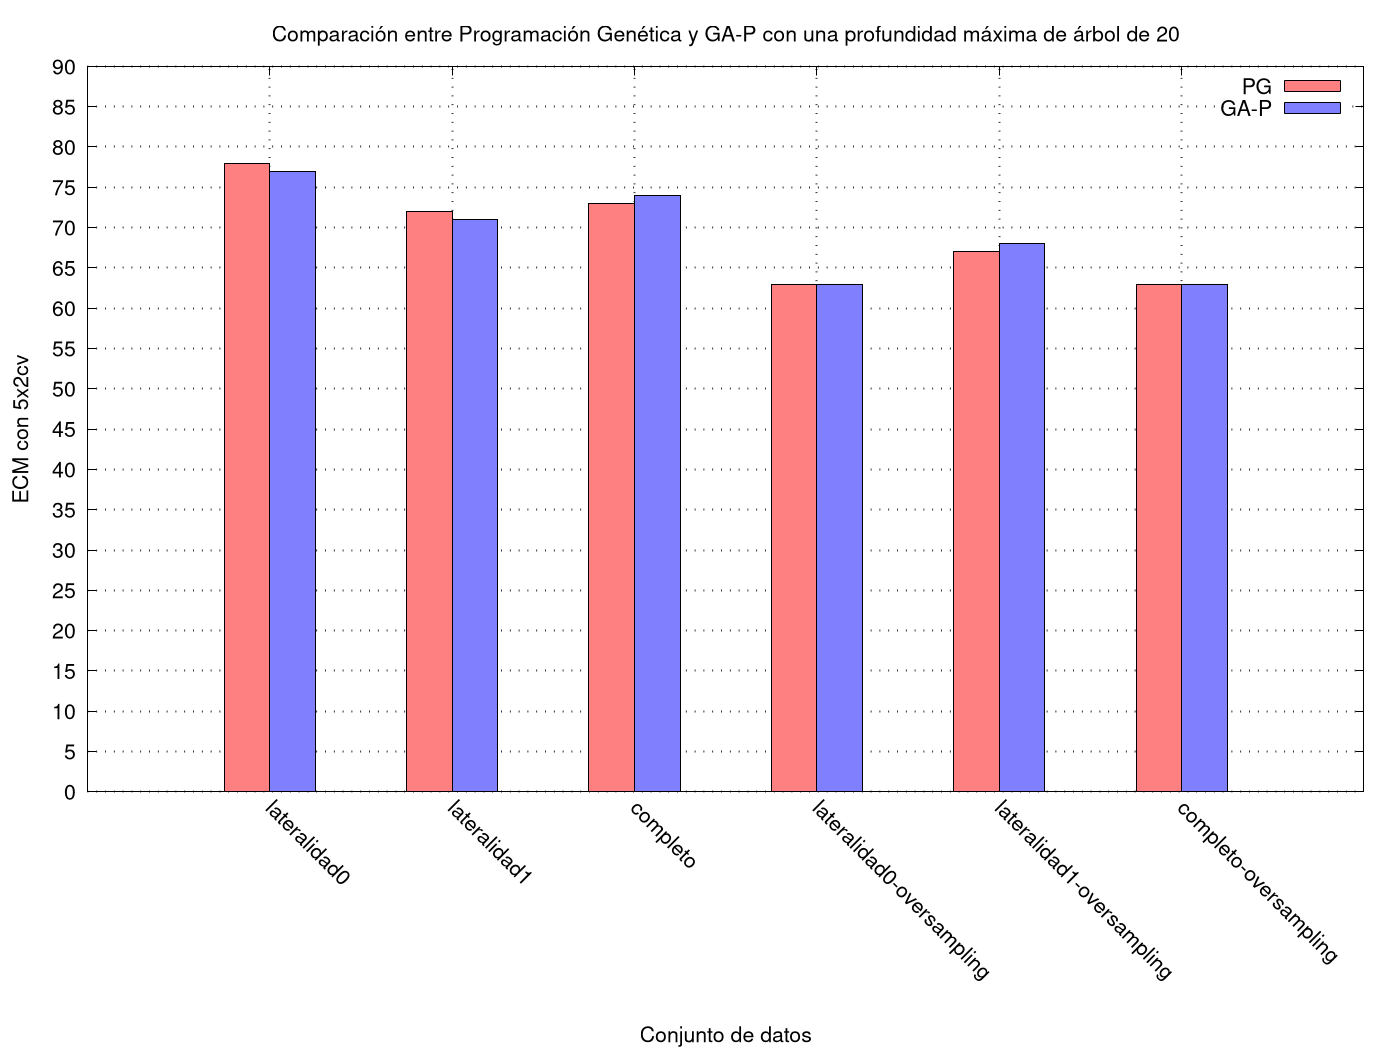
\includegraphics[width=0.7\textwidth]{analisis/comparacion_pg_gap_20.png}
	  \caption{Comparación entre PG y GA-P con profundidad máxima de 20 nodos.}\label{fig:cmp_pg_gap_20}

\end{figure}

\begin{figure}[H]
    \centering
	  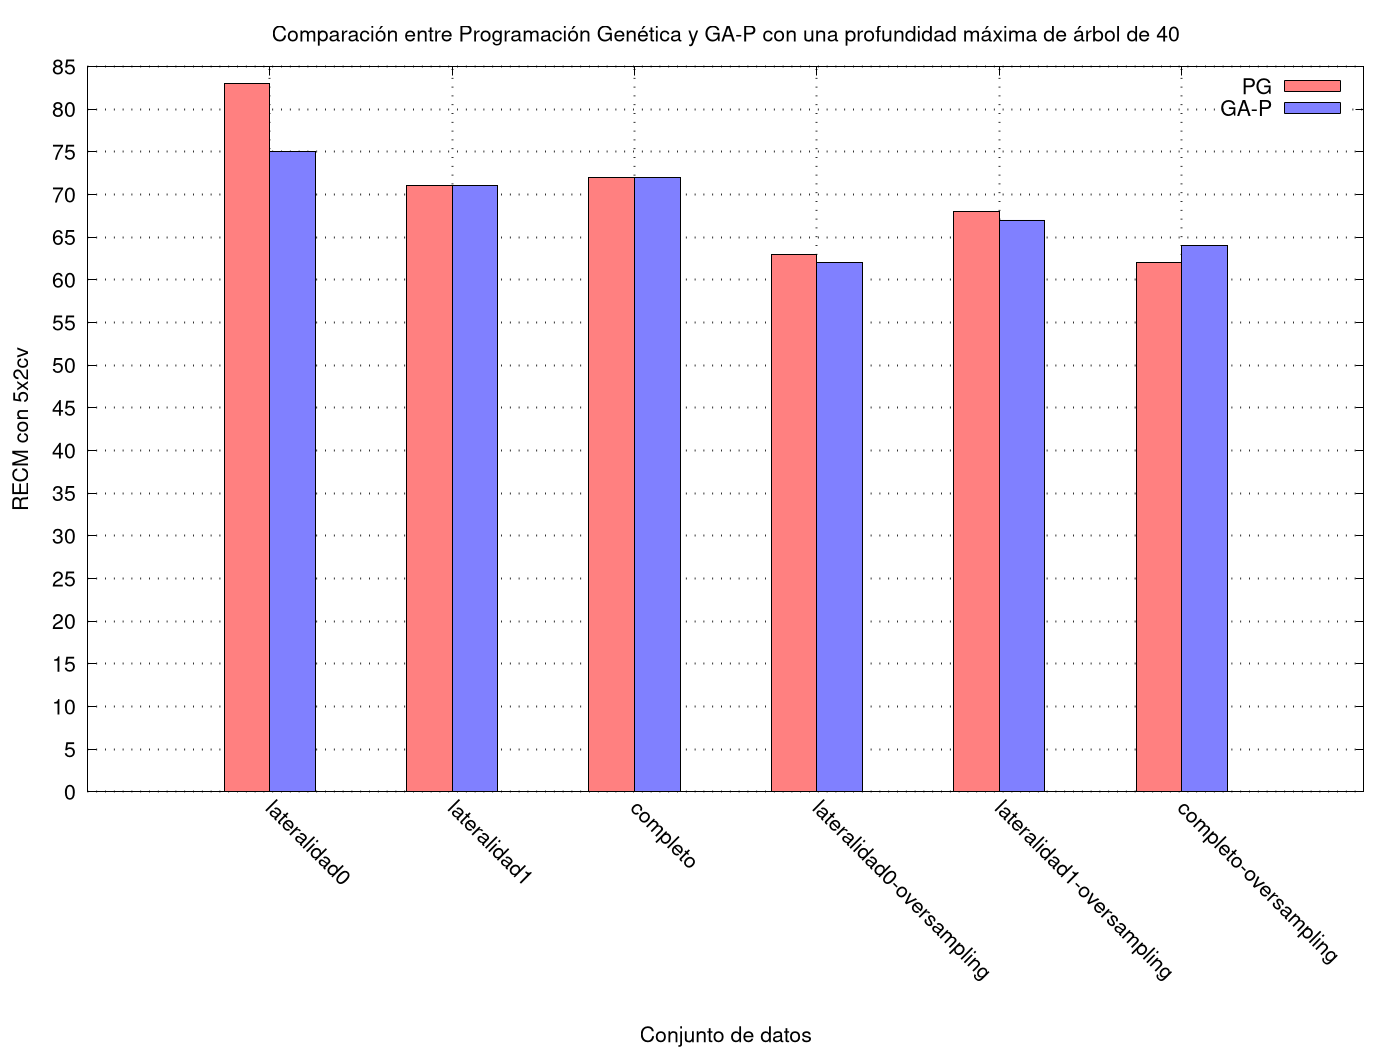
\includegraphics[width=0.7\textwidth]{analisis/comparacion_pg_gap_40.png}
	  \caption{Comparación entre PG y GA-P con profundidad máxima de 40 nodos.}\label{fig:cmp_pg_gap_40}

\end{figure}

\begin{figure}[H]
    \centering
	  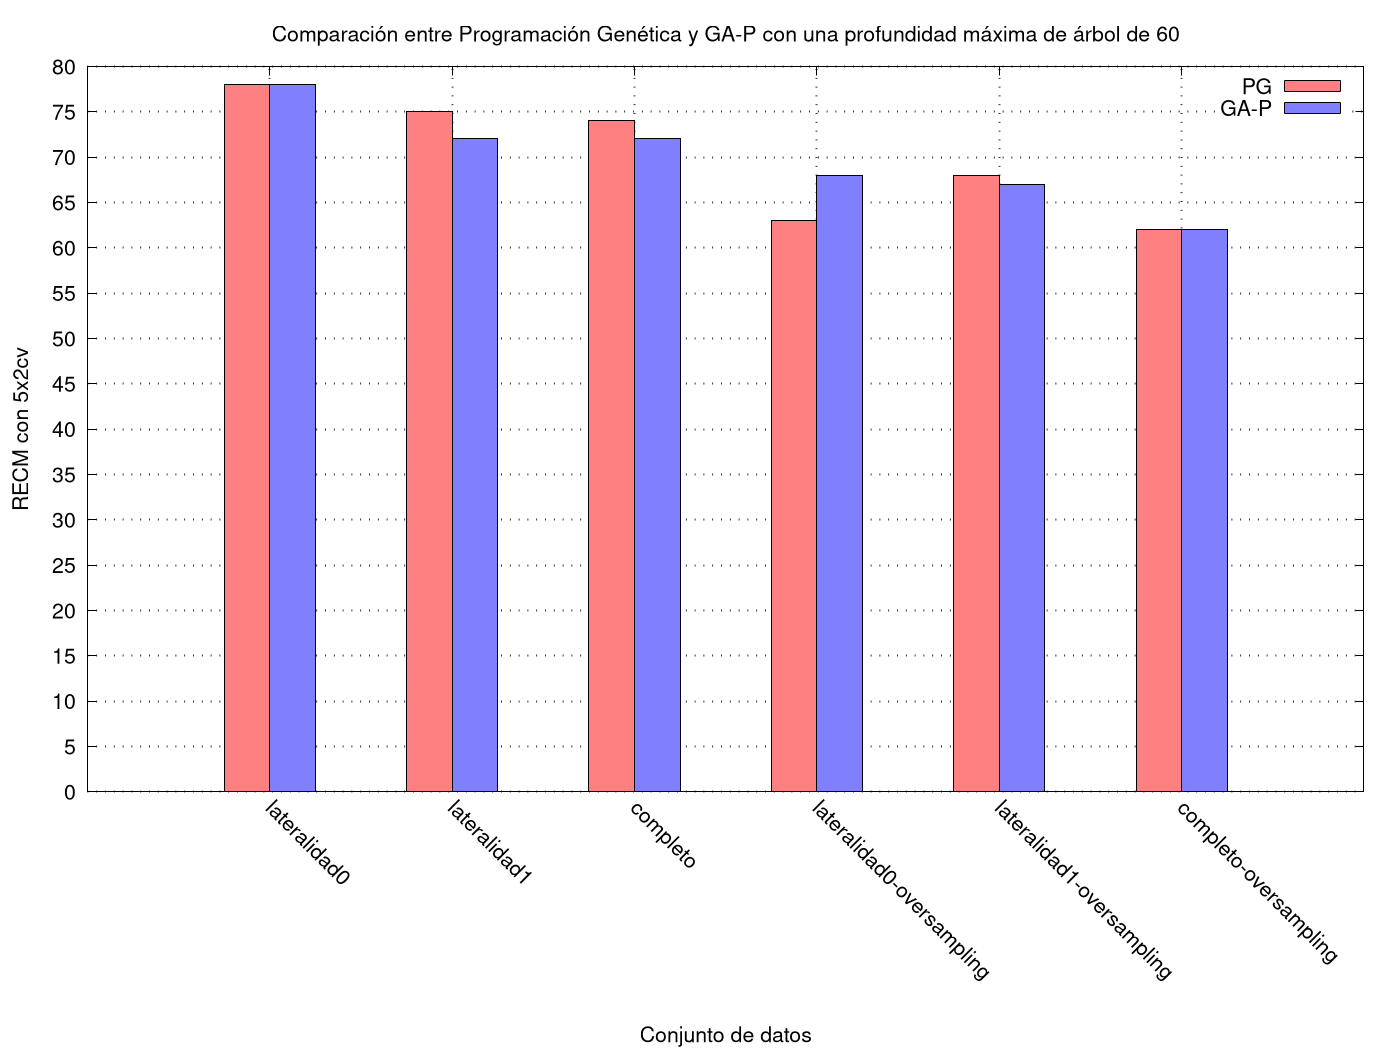
\includegraphics[width=0.7\textwidth]{analisis/comparacion_pg_gap_60.png}
	  \caption{Comparación entre PG y GA-P con profundidad máxima de 60 nodos.}\label{fig:cmp_pg_gap_60}
\end{figure}



Las tablas \ref{table:resumen_l0}, \ref{table:resumen_l1} y \ref{table:resumen_completo} e imágenes \ref{fig:cmp_pg_gap_20}, \ref{fig:cmp_pg_gap_40} y \ref{fig:cmp_pg_gap_60} nos muestran como la mejora de GA-P se nota especialmente en los conjuntos de datos sin sobremuestreo, mientras que en los resultados con sobremuestreo esta diferencia es más pequeña, lo que nos lleva a pensar que GA-P es más versátil para conjuntos de datos donde existen pocas muestras para algunas etiquetas, adaptándose mejor que Programación Genética para problemas de regresión simbólica al implementar la mejora de nichos y aprender mejor la fórmula obtenida, ya que Programación Genética si que necesita más cantidad de datos para aprender la fórmula.

\subsubsection{Comparación de resultados del conjunto de datos original y del conjunto de datos con sobremuestreo}

Con respecto a los resultados obtenidos con el conjunto de datos original y el conjunto con datos sintéticos, podemos ver como claramente se consigue una mejora en los resultados:

% TODO insertar imágenes

\begin{figure}[H]
    \centering
	  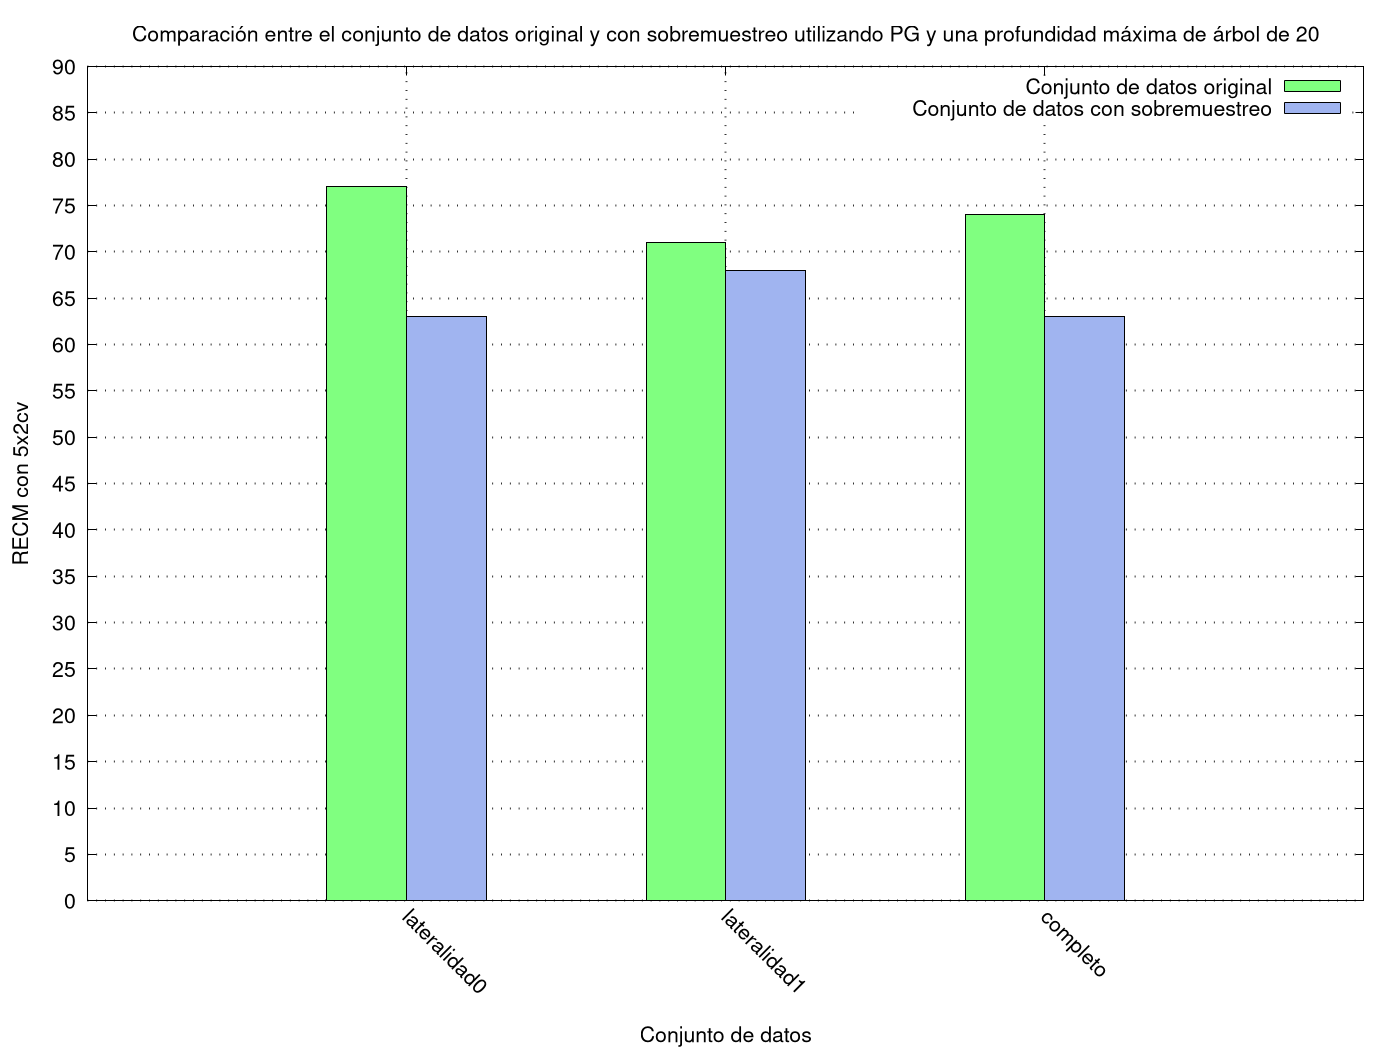
\includegraphics[width=0.7\textwidth]{analisis/comparacion_over_pg_20.png}
	  \caption{Comparación entre el conjunto de datos original y con sobremuestreo con PG y profundidad máxima de 20 nodos.}\label{fig:cmp_pg_over_20}

\end{figure}

\begin{figure}[H]
    \centering
	  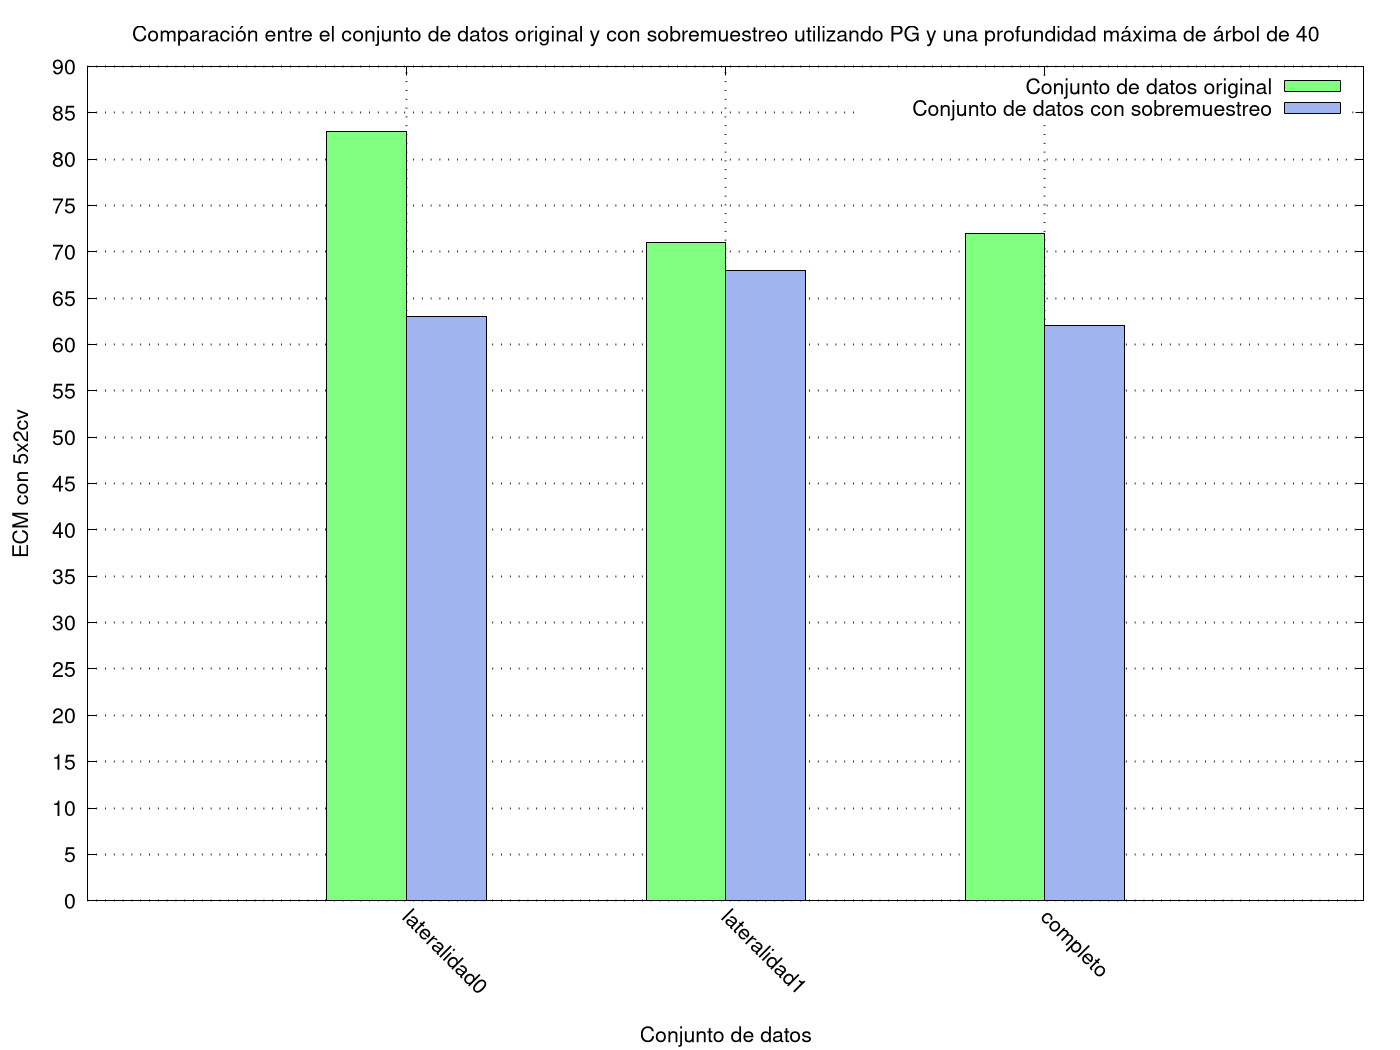
\includegraphics[width=0.7\textwidth]{analisis/comparacion_over_pg_40.png}
	  \caption{Comparación entre el conjunto de datos original y con sobremuestreo con PG y profundidad máxima de 40 nodos.}\label{fig:cmp_pg_over_40}

\end{figure}

\begin{figure}[H]
    \centering
	  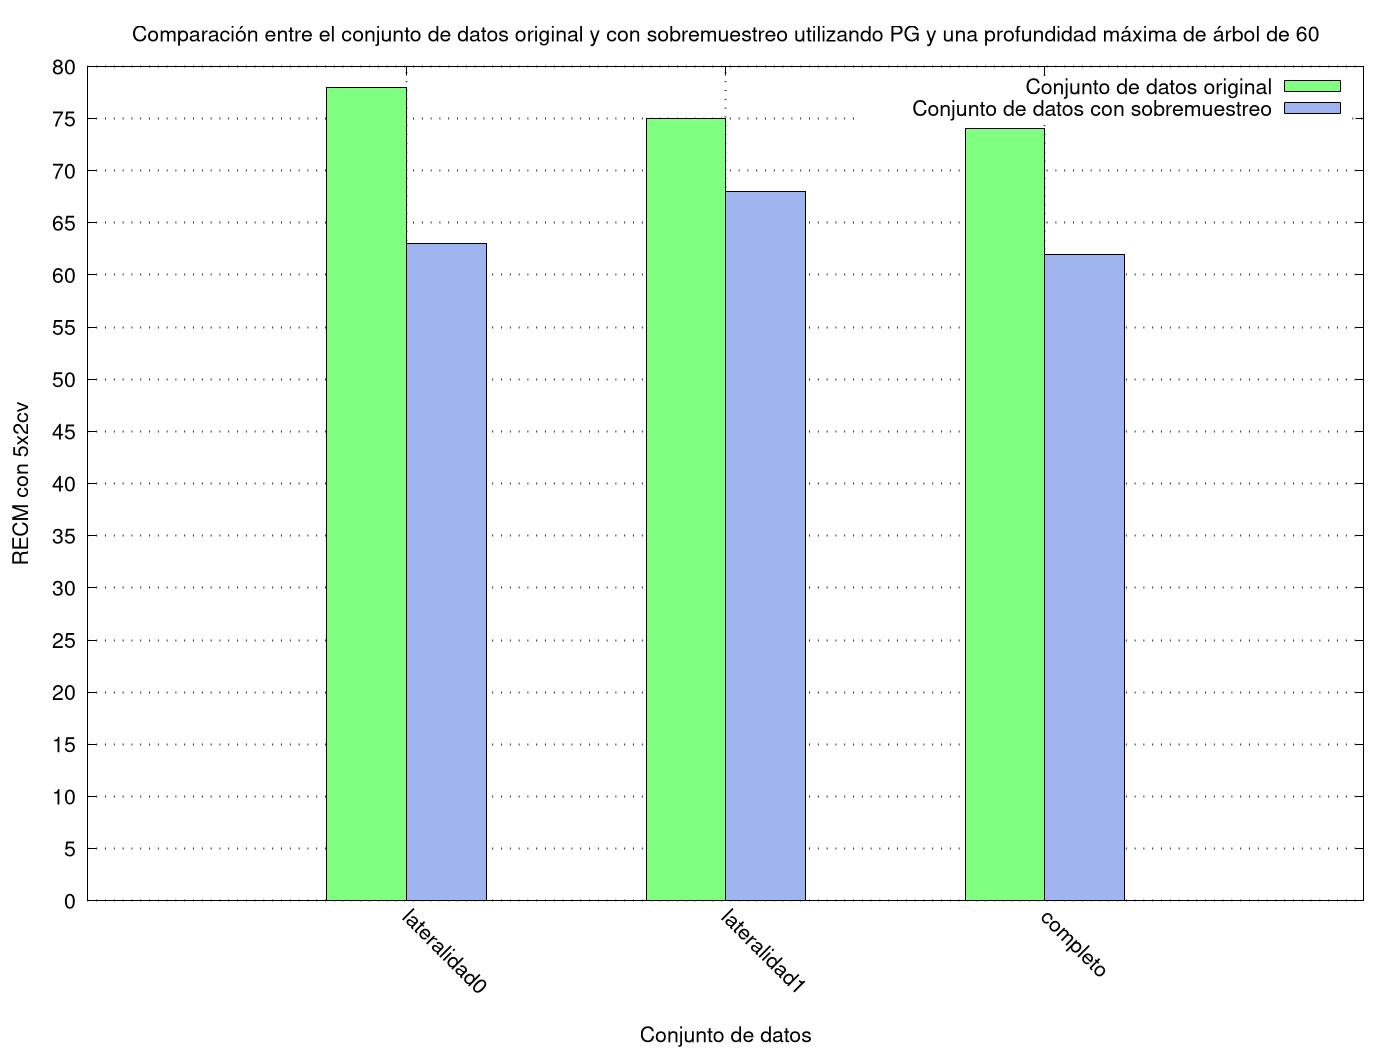
\includegraphics[width=0.7\textwidth]{analisis/comparacion_over_pg_60.png}
	  \caption{Comparación entre el conjunto de datos original y con sobremuestreo con PG y profundidad máxima de 60 nodos.}\label{fig:cmp_pg_over_60}

\end{figure}

Estos cambios también son notables sobre GA-P:

\begin{figure}[H]
    \centering
	  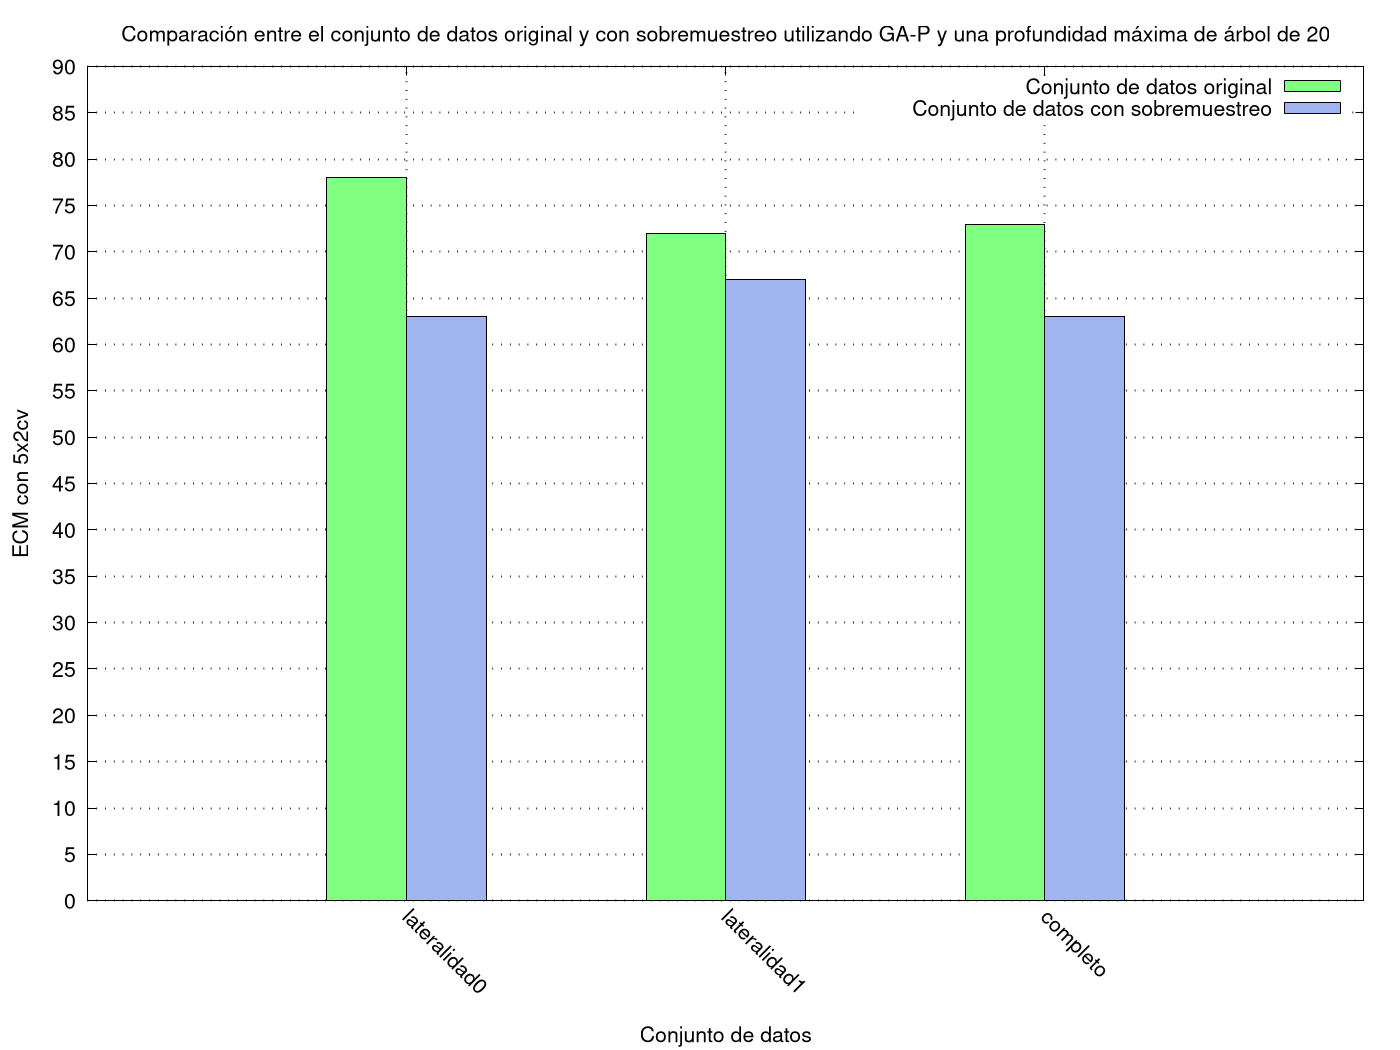
\includegraphics[width=0.7\textwidth]{analisis/comparacion_over_gap_20.png}
	  \caption{Comparación entre el conjunto de datos original y con sobremuestreo con GA-P y profundidad máxima de 20 nodos.}\label{fig:cmp_gap_over_20}

\end{figure}

\begin{figure}[H]
    \centering
	  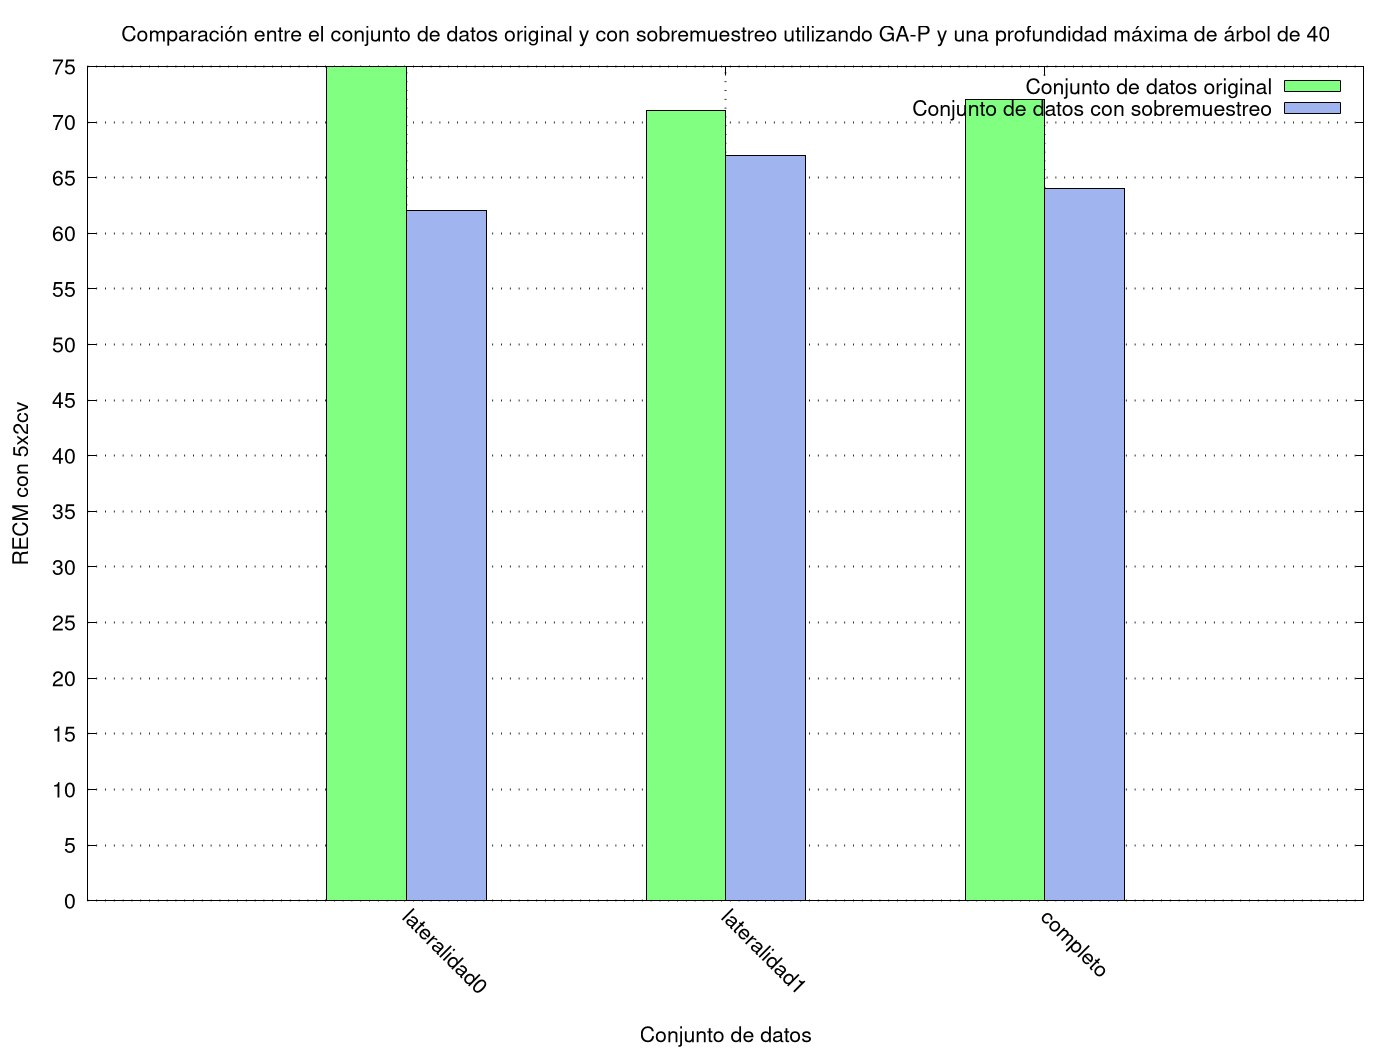
\includegraphics[width=0.7\textwidth]{analisis/comparacion_over_gap_40.png}
	  \caption{Comparación entre el conjunto de datos original y con sobremuestreo con GA-P y profundidad máxima de 40 nodos.}\label{fig:cmp_gap_over_40}

\end{figure}

\begin{figure}[H]
    \centering
	  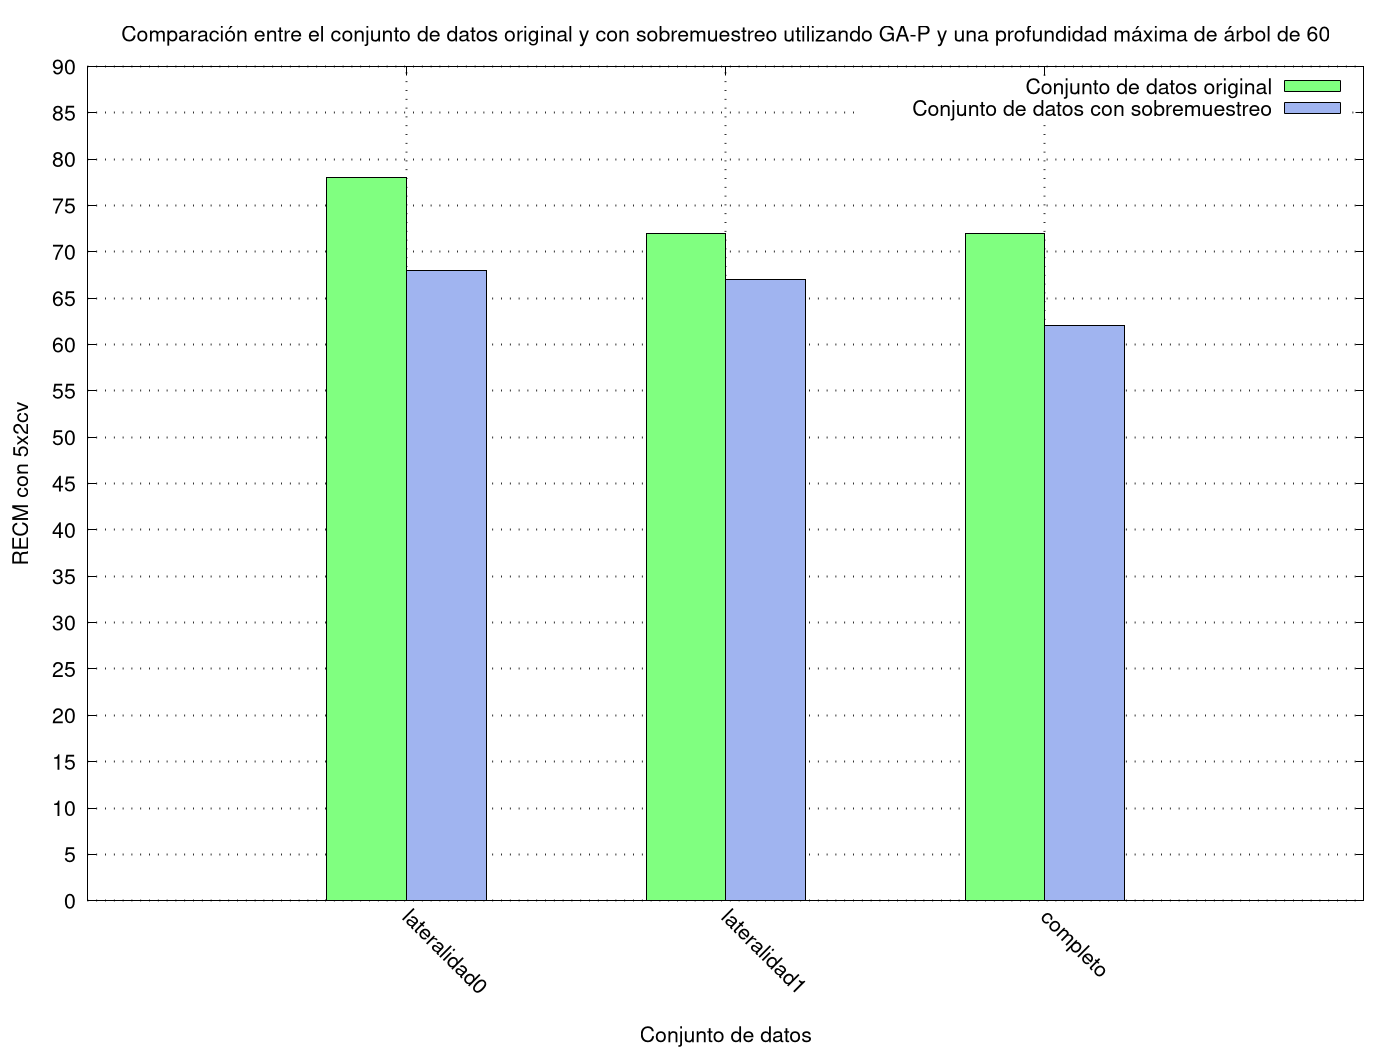
\includegraphics[width=0.7\textwidth]{analisis/comparacion_over_gap_60.png}
	  \caption{Comparación entre el conjunto de datos original y con sobremuestreo con GA-P y profundidad máxima de 60 nodos.}\label{fig:cmp_gap_over_60}

\end{figure}

\subsubsection{Análisis de las expresiones obtenidas y mejores expresiones}

\subsubsection{Comparación con el estado del arte}




\newpage
